\documentclass[12pt]{article}
\usepackage{latexsym,amsmath,amssymb,tabu,CJKutf8,bm,graphicx}
\usepackage{caption,float}
\usepackage{multirow,booktabs,diagbox}
\textwidth 6.5in \textheight 9in \oddsidemargin 0pt \topmargin -8pt
\pagestyle{plain}

\begin{document}
\begin{CJK}{UTF8}{gkai}
    \title{SCFT$-$VEM}
    \date{\today}
    \author{王鑫}
    \maketitle
    \section{网格数据结构:}    
    \subsection{方形网格数据结构:}
    \begin{figure}[H]
     \centering
     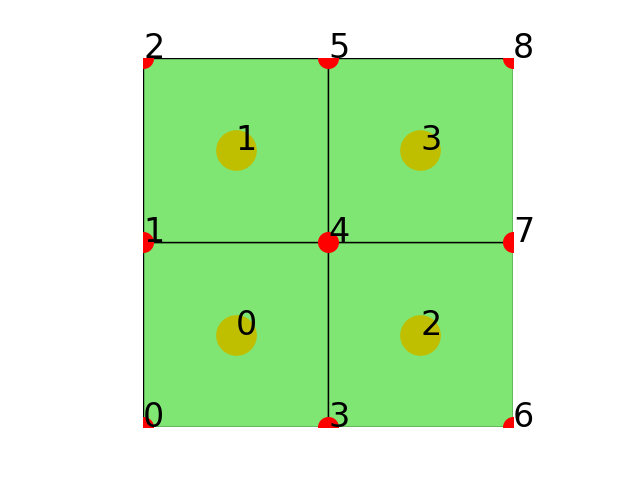
\includegraphics[width=8cm]{Figure_2.png}
     \caption{}  		
     \end{figure}


    相应的node和cell:\\

   \begin{figure}[H]
    \centering   
    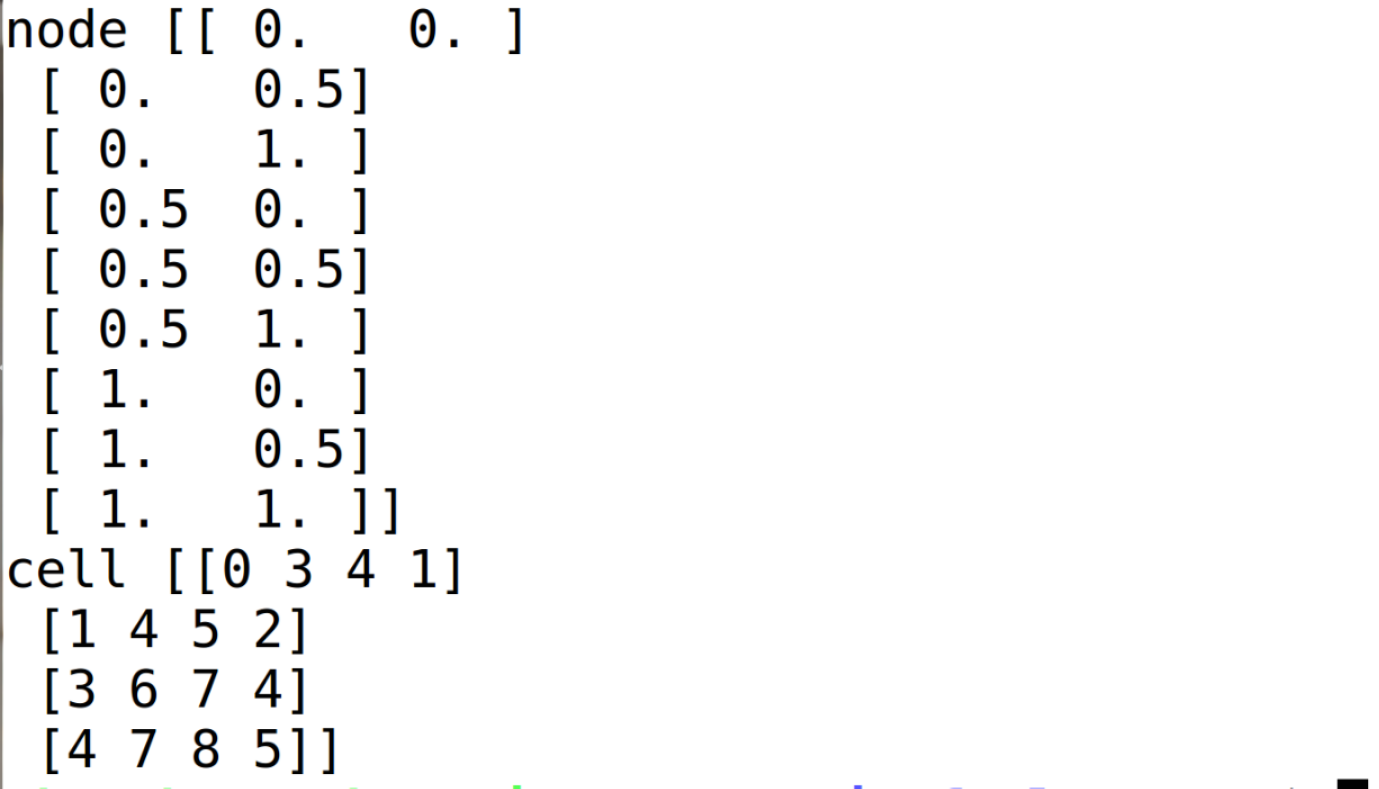
\includegraphics[width=8cm]{4.png}
    \caption{}
    \end{figure}
    
   \subsection{多边形网格数据结构:}

     \begin{figure}[H]
     \centering
     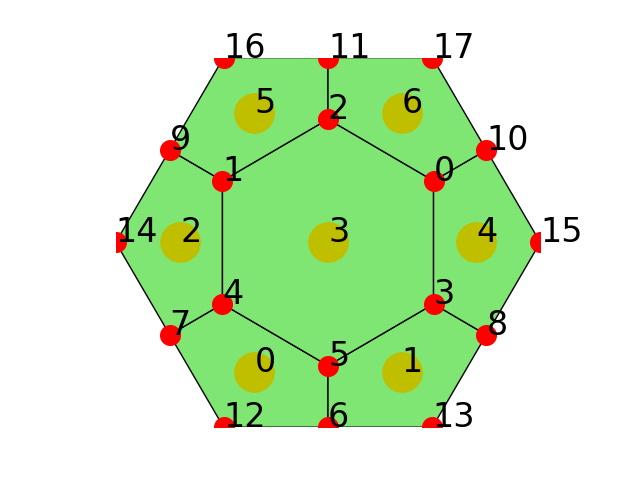
\includegraphics[width=10cm]{Figure_1.png}
     \caption{}  		
     \end{figure}

    相应的node和cell:\\

   \begin{figure}[H]
    \centering   
    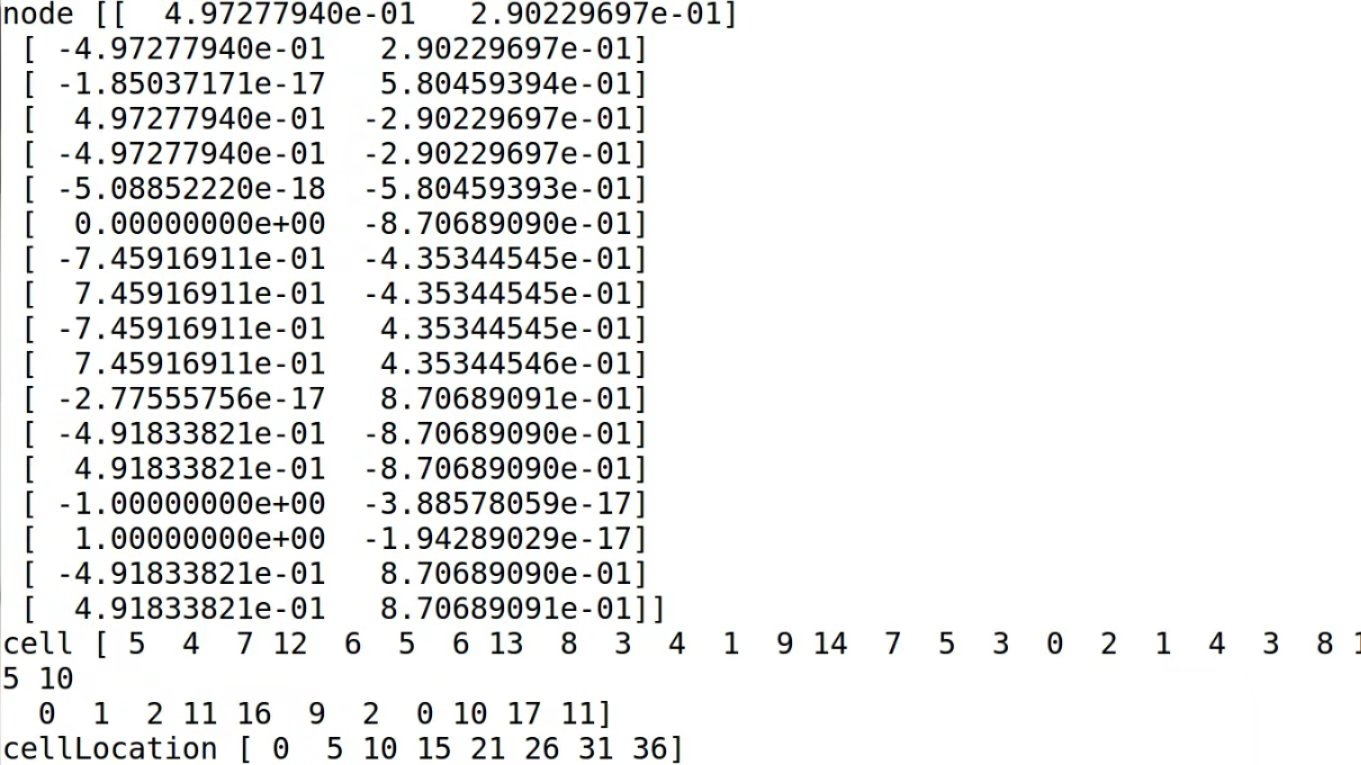
\includegraphics[width=10cm]{1.jpg}
    \caption{}
    \end{figure}
    
    \section{虚单元自洽场模拟}
    
     \subsection{虚单元理论}
    
  \subsubsection{模型:泊松方程}
    
     \begin{equation}\label{eq:dirichlet}
     \begin{cases}
     -\Delta u =f,\qquad  in\quad \Omega.\\
     u=g_D,\qquad on \quad\partial \Omega 
     \end{cases}
     \end{equation}
     $\Omega $是$\mathbb{R}^2$中的多边形区域\\
     
     找到$ u \in H_{g_D}^{1}(\Omega)$:
     \begin{equation}
     (\nabla u,\nabla v)=(f,v) ,\qquad \forall v \in H_0^1(\Omega)
     \end{equation}
     
     其中
     \begin{gather}
     H_{g_D}^{1}=\{u \in H^1(\Omega)\text{且}u|_{ \partial \Omega} = g_D\}\\
     H_{0}^{1}=\{v \in H^1(\Omega)\text{且}u|_{ \partial \Omega} =0\}
     \end{gather}
     
      \subsubsection{二维局部虚单元空间 $\mathcal V_k(E)$}
     \begin{table}[H]
     	\centering
     \begin{tabular}{ cc }   
     	\hline
     	符号 & 含义 \\
     	\hline
     	$E$ & 多边形,可以是非凸的 \\
     	
     	$\Omega$ & 二维有界区域. $\Omega$$\subset$ $\mathbb{R}^2$, $\Omega$ =$\cup_{E\in \mathcal{P}_h}E$ \\
     
     	$V_i$ & $E$ 上逆时针顺序标记的顶点,其中 $i = 1,\cdots, N^V,N^V$ 表示 $E$ 的总的顶点数目 \\
     	
     	$e_i$ & $E$ 中连接 $V_i$ 和 $V_{i+1}$ 的边. 允许两条相邻的边构成 $180$ 度角 \\
     	\hline
     \end{tabular}
     \end{table}
     
    定义函数 $v_h$, $v_h\in\mathcal V_k(E)$ 且满足如下性质:\\
    \\
    $1$) $v_h$ 在 $E$ 的每条边 $e$ 上是一个次数 $\le k$ 多项式, i.e.,$v_h|_e \in \mathcal P_k(e)$\\
    $2$) $v_h$ 在 $E$ 的边界 $\partial E$ 上是全局连续的,i.e.,$v_h|_{\partial E} \in \mathcal C^0(\partial E)$\\
    $3$) $\Delta v_h$ 在 $E$ 内是一个次数 $\le k - 2$ 的多项式, i.e., $\Delta v_h \in \mathcal P_{k-2}(E)$\\
    
    所以 $\mathcal{P}_k(E)$ 是 $V_k(E)$ 子空间. \\
    
    $v_h\in \mathcal V_k(E)$ 的自由度定义如下:\\
    \\
    (1) $v_h$ 在 $E$ 的所有顶点处的函数值\\
    (2) $v_h$ 在 $E$ 的每条除顶点以外的 $k-1$ 个 Gauss-Lobatto 积分点处函数值 \\ 
    (3) $v_h$ 在单元 $E$ 内部与 $\mathcal P_{k-2}(E)$ 中所有单项式 $m_\alpha$ 的乘积的积分平均值, $$ \frac{1}{|E|}\int_E v_h m_\alpha, \quad \alpha = 1, \ldots, n_{k-2}$$
    其中 $n_{k-2} = \dim \mathcal P_{k-2}(E)$\\
    
    易知 $\mathcal V_k(E)$ 的维数为 \\
    \begin{equation}
    N^{dof} = \text{dim} \mathcal V_k(E) = N^V + N^V(k - 1) + n_{k - 2} = N^Vk+ \frac{(k-1)k}{2}.
    \end{equation}
    
    定义从 $V_k(E)$ 到 $\mathbb{R}$ 的算子 $dof_i$ \\
    \begin{equation}
    dof_{i}(v_h) = v_h \text{的第} i \text{个自由度}, \,\ i,j = 1,\cdots, N^{dof} 
    \end{equation}
    
    其中 $N^{dof} := dimV_k(E)$ \\
    
    对于基函数 $\varphi_j \in V_k(E)$ \\
    \begin{equation}
    dof_{i}(\varphi_j) = \delta_{ij},\quad i,j = 1,\cdots,N^{dof} 
    \end{equation}
    
    由于边界自由度在每条边界上都是唯一的次数 $\le k$ 的多项式. 因此, 可以定义全局虚单元空间 $V_h \subset H_0^1(\mathcal D)$ \\
    \begin{equation*}
    V_h := {v_h \in H_0^1(\mathcal D) : \text{对所有} E\in\mathcal{P}_h \text{满足} v_h|_E \in V_k(E)}
    \end{equation*}
    
    $v_h$ 有以下的全局自由度: \\
    \\
    1) $v_h$ 在剖分后的区域的所有内部顶点处的值 \\
    2) $K + 1$ 点 $Guass-Lobatto$ 型求积公式在每条内部边 $e$ 上有 $k - 1$ 个内部积分值, $v_h$ 在所有边内部积分点处的积分值 \\  
    3) 每一个多边形 $E$ 内部的 $n_{k - 2}$个自由度\\
    \begin{equation}
    \frac{1}{|E|}\int_{E}v_hm_{\alpha},\,\ \alpha = 1,\cdots,n_k
    \end{equation}
    
    其中 $n_{k-2} = dim\mathcal{P}_{k - 2}(E)$\\
    
   \subsubsection{计算单元刚度矩阵}
  
    定义在多边形 $E$ 上的 $Laplace$ 算子的单元刚度矩阵\\
    \begin{equation}
    \mathbf(K_E)_{ij} = (\nabla\varphi_i, \nabla\varphi_j)_{0,E},\quad i,j = 1,\cdots,N^{dof}
    \end{equation}
    其中 $\varphi_i \in V_k(E)$ 是 $(2.2)$ 定义的基函数. \\
    
    VEM方法的好处:\\
    
    既不要求使用积分公式也不需要基函数的近似表达式\\
    
     \subsubsection{投影算子 $\Pi^{\nabla}$}
    
    定义 $\Pi^\nabla: \mathcal V_k(E)\rightarrow \mathcal{P}_k(E)$ 如下: 给定  $ v_h \in
    \mathcal V_k(E)$, 找到 $\Pi^\nabla v_h \in \mathcal{P}_k(E)$ 满足: \\
    \begin{equation}
    (\nabla \Pi^\nabla v_h, \nabla p_k) = (\nabla v_h, \nabla p_k), \forall p_k\in\mathcal{P}_k(E)
    \end{equation}
    
    如上所示,满足性质 $(3.2)$ 的 $\Pi^{\nabla}v_h$ 仅为常量,为了确定这个常量可以定义投影: \\
    $ P_0: \mathcal V_k(E) \rightarrow
    \mathcal{P}_0(E)$:
    
    \begin{equation}
    P_0(\Pi^\nabla v_h - v_h) = 0
    \end{equation}
    
    具体定义如下: \\
    \begin{equation}
    \begin{aligned}
    P_0 v_h :=& \frac{1}{N^V}\sum_{i=1}^{N^V} v_h(\mathbf x_i)\text{, for } k=1 \\
    P_0 v_h :=& \frac{1}{|E|} \int_{E}v_h = \frac{1}{|E|} (1, v_h)_E\text{, for } k\geq 2
    \end{aligned}
    \end{equation}
    
    其中 $\frac{1}{|E|} (1, v_h)_E$ 为 $v_h$ 在 $E$ 内部自由度处的值.\\
    
    对于一个给定的 $v_h \in V_k(E)$, 下面展示只使用 $v_h$ 的自由度计算 $\Pi^{\nabla}v_h$ 的过程. \\
    
    因为 $\mathcal M _k(E)$ 是 $\mathcal P_k(E)$ 的一组基,所以让符合性质 $(3.2)$ 的 $p_k$ 只在 $\mathcal M _k(E)$ 范围内变化,即 \\
    \begin{equation}
    (\nabla m_{\alpha}, \nabla(\Pi^{\nabla}v_h) - v_h)_{0,E} = 0,\,\ \alpha = 1,2,\cdots, n_k
    \end{equation}
    
    因为 $\Pi^{\nabla}v_h \in \mathcal P_k(E)$,所以 $\Pi^{\nabla}v_h$ 也可以由基 $\mathcal M_k(E)$ 表示\\
    \begin{equation}
    \Pi^\nabla v_h = \sum_{\beta = 1}s^{\beta}m_\beta
    \end{equation}
    
    把公式 $(3.6)$ 代入公式 $(3.5)$, 得 \\
    \begin{equation}
    \sum_{\beta = 1}^{n_k}s^{\beta}(\nabla m_{\alpha},\nabla m_{\beta})_{0,E} = (\nabla m_{\alpha, \nabla v_h})_{0,E}
    \end{equation}
    
    公式 $(3.7)$ 是由含 $n_k$ 个未知数 $s^{\beta} = s^{\beta}(v_h)$ 的 $n_k$ 个方程组成的线性系统.然而当 $\alpha = 1$ 时, $m_{\alpha} \equiv 1$, 从而方程 $3.7$ 变为 $0 = 0$, 使得方程的解是不确定的. 为了消除这种不确定性,条件 $(3.3)$ 增加一个线性方程: \\
    \begin{equation}
    \sum_{\beta = 1}^{n_k}s^{\beta}P_0m_{\beta} = P_0v_h
    \end{equation}
    那么结合 $(3.7)$ 和 $(3.8)$, 线性方程组可以写成 \\
    \begin{equation*}
    \left[ \begin{array}{cccc}
    P_0m_1 & P_0m_2  &\cdots&P_0m_{n_k} \\
    0 & (\nabla m_2,\nabla m_2)_{0,E} & \cdots & (\nabla m_2,\nabla m_{n_k})_{0,E} \\
    \vdots & \vdots & \ddots & \vdots\\
    0& (\nabla m_{n_k},\nabla m_2)_{0,E} & \cdots & (\nabla m_{n_k},\nabla m_{n_k})_{0,E}
    \end{array} \right]
    \left[ \begin{array}{c}
    s^1\\
    s^2\\
    \vdots\\
    s^{n_k}
    \end{array} \right]
    = \left[\begin{array}{c}
    P_0v_h\\
    (\nabla m_2,\nabla v_h)_{0,E} \\
    \vdots\\
    (\nabla m_{n_k},\nabla v_h)_{0,E} 
    \end{array}\right]
    \end{equation*}
    
    换一种写法,也就是 \\
    \begin{equation}
    G\underline{s} = \underline{b}
    \end{equation}
    
    其中 \\
    \begin{equation}
    G := \begin{bmatrix}
    P_0m_1 & P_0m_1 &\cdots&P_0m_{n_k} \\
    0 & (\nabla m_2,\nabla m_2)_{0,E} & \cdots & (\nabla m_2,\nabla m_{n_k})_{0,E} \\
    \vdots & \vdots & \ddots & \vdots\\
    0& (\nabla m_{n_k},\nabla m_2)_{0,E} & \cdots & (\nabla m_{n_k},\nabla m_{n_k})_{0,E}
    \end{bmatrix}\\
    \end{equation}
    \begin{equation}
    \underline b := \begin{bmatrix}
    P_0v_h\\
    (\nabla m_2,\nabla v_h)_{0,E} \\
    \vdots\\
    (\nabla m_{n_k},\nabla v_h)_{0,E} 
    \end{bmatrix}
    \end{equation}
    
    假定 $E$ 上的多项式的积分是可以计算的, 公式 $(3.10)$ 中的矩阵 $G$ 是可以计算的. \\

...\\

    \subsection{有限元和虚单元数值方法对比}
            
       在本小节我们应用有限元和虚单元数值方法分别对泊松方程求解\\
       
       两种方法数值实验中计算区域相同\\
       
       当初始网格尺寸$h=0.4$时,网格顶点个数NN为19,单元个数NC为24,边的个数NE为40.\\
       
       故有限元方法中自由度为:\\
        \begin{equation}
        N_{dof}=NN=19
        \end{equation}
        
         故虚单元方法中自由度为:\\
         \begin{equation}
         N_{dof}=NN+NN*(k-1)+dim(P_{k-2}) , k\text{为多项式次数}      
         \end{equation}
         
         故$k=1$时\\
         \begin{equation}
         N_{dof}=NN=19   
         \end{equation} 
       
         
         
         当初始网格尺寸$h=0.2$时,网格顶点个数NN为77,单元个数NC为125,边的个数NE为201.\\
         
         故有限元方法中自由度为:\\
         \begin{equation}
         N_{dof}=NN=77
         \end{equation}
         
         故虚单元方法中自由度同上为:\\
         \begin{equation}
         N_{dof}=NN=77
         \end{equation}
         
       
       
       \subsubsection{有限元数值结果}
       \begin{figure}[H] 
       	\centering
       	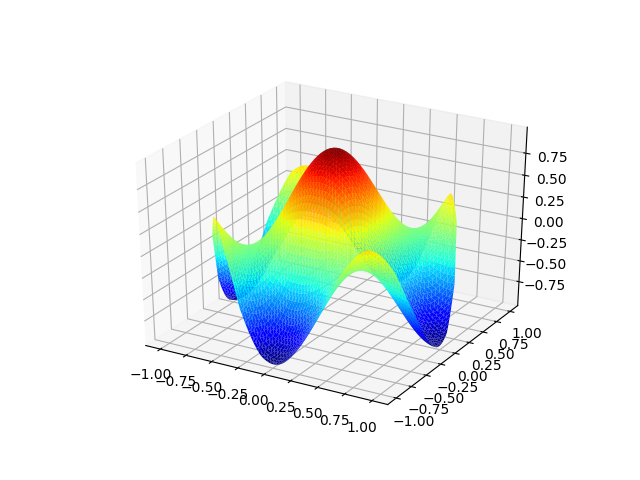
\includegraphics[width=10cm]{Figure_3.png}
       	\caption{有限元数值解}
       \end{figure}
       
       \begin{figure}[H] 
       	\centering
       	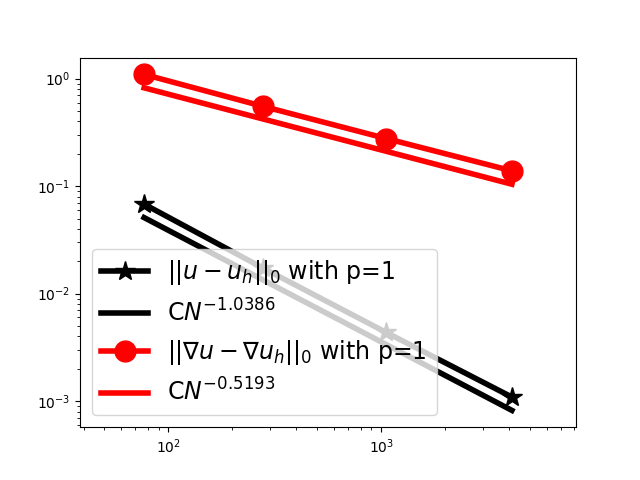
\includegraphics[width=10cm]{Figure_2-1.png}
       	\caption{有限元误差}
	  \end{figure}
        
        \subsubsection{虚单元数值结果}
        
        对虚单元的边界边进行了加密, $n$为每条边界边加密点的个数\\
        
        初始网格结构为:\\
        \begin{figure}[H] 
        	\centering
        	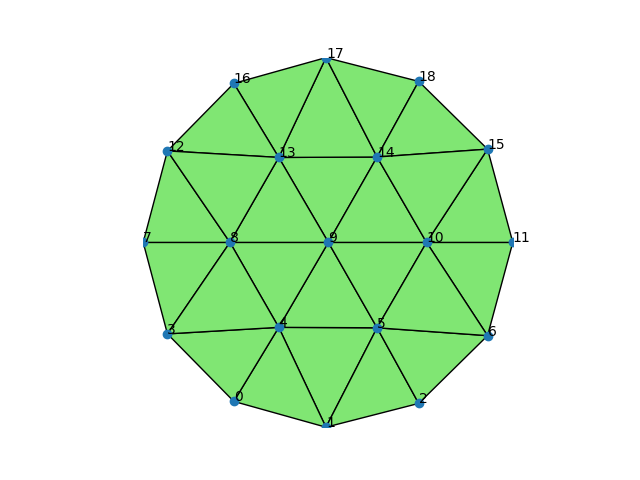
\includegraphics[width=10cm]{0.png}
        	\caption{$h=0.4$时网格结构}
        \end{figure}
        
        当网格边界单元的每条边界边加了两个点时,网格数据结构为:\\
        \begin{figure}[H] 
        	\centering
        	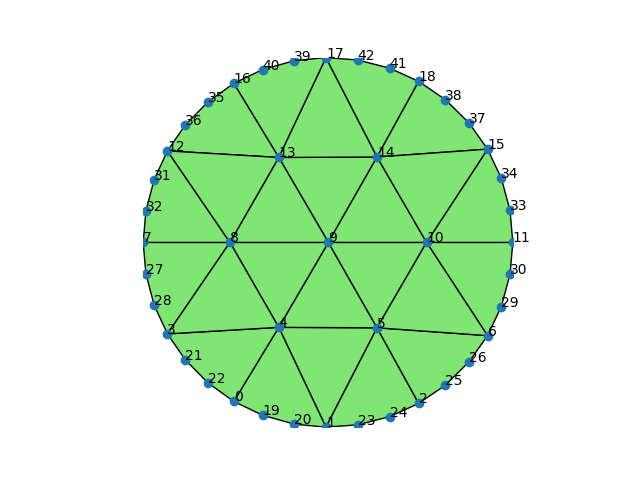
\includegraphics[width=10cm]{aa.png}
        	\caption{$h=0.4$且$n=2$的网格结构}
        \end{figure}
        \
         \begin{figure}[H] 
           \centering
           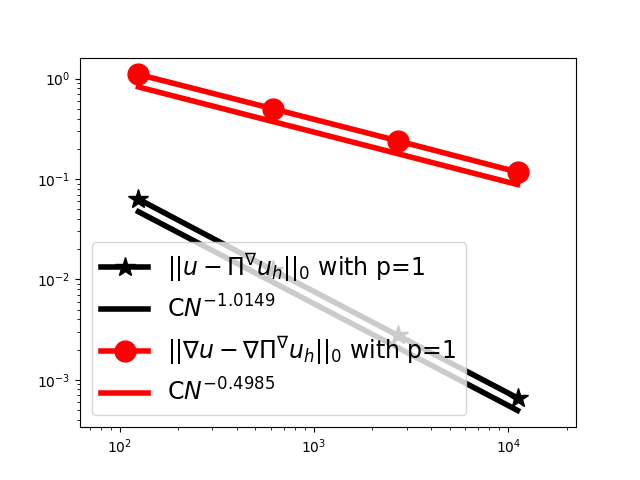
\includegraphics[width=10cm]{10e.png}
           \caption{虚单元误差}
         \end{figure}

             
             \subsubsection{误差对比}           
          
             \begin{table}[H]
           	    \centering
                \begin{tabular}{ccccc}
             	\toprule
             	\multirow{3}*{h} &  \multicolumn{2}{c}{FEM} & \multicolumn{2}{c}{VEM}\\
             	\cmidrule(lr){2-3} \cmidrule(lr){4-5}
             	\multicolumn{3}{c}{ }&\multicolumn{2}{c}{$n=1$}\\ 
             	\cmidrule(lr){4-5}       
             	& $error_{L^2}$ &	$error_{H^1}$&$ error_{L^2} $ &  $ error_{H^1} $	   \\
             	\midrule
             	0.4&3.06353371e-01&2.3634064e+00&2.9155471e-01&2.34196857e+00\\
             	0.2&6.80075013e-02&1.0959139e+00&6.36205561e-02&1.09589832e+00 \\
             	0.1&1.39537223e-02&5.01866396e-01&1.26657361e-02 &5.01190429e-01 \\
             	0.05&3.16847981e-03&2.40128919e-01&2.83066896e-03 &2.39918815e-01 \\
             	\bottomrule
               \end{tabular} 
             \end{table}
          
             \begin{table}[H]
             	\centering
             \begin{tabular}{ccccc}
           	\toprule
           	\multirow{3}*{h} &   \multicolumn{4}{c}{VEM}\\
           	\cmidrule(lr){2-5} 
           	\multicolumn{3}{c}{$n=2$ }&\multicolumn{2}{c}{$n=3$}\\ 
           	\cmidrule(lr){2-3}  \cmidrule(lr){4-5}     
           	& $error_{L^2}$ &	$error_{H^1}$&$ error_{L^2} $ &  $ error_{H^1} $	   \\
           	\midrule
           	0.4&2.90864600e-01&2.35650640e+00&2.9081108e-01&2.36261577e+00\\
           	0.2&6.31297281e-02&1.09856418e+00&6.29873642e-02&1.09968281e+00 \\
           	0.1&1.25148788e-02&5.01530776e-01&1.24695914e-02 &5.01683656e-01 \\
           	0.05&2.79279524e-03&2.39972869e-01&2.78160688e-03 &2.39998607e-01 \\
           	
           	\bottomrule
             \end{tabular}
           \end{table} 
             
             
         \begin{table}[H]
         	\centering    
        \begin{tabular}{ccccc}
        	\toprule
        	\multirow{3}*{h} &   \multicolumn{4}{c}{VEM}\\
        	\cmidrule(lr){2-5} 
        	\multicolumn{3}{c}{$n=4$ }&\multicolumn{2}{c}{$n=5$}\\ 
        	\cmidrule(lr){2-3}  \cmidrule(lr){4-5}     
        	& $error_{L^2}$ &	$error_{H^1}$&$ error_{L^2} $ &  $ error_{H^1} $	   \\
        	\midrule
        	0.4&2.9082541e-01&2.36561809e+00&2.9084788e-01&2.3672956e+00\\
        	0.2&6.29294389e-02&1.10023322e+00&6.29022306e-02&1.10054133e+00\\
        	0.1&1.24504173e-02&5.01760363e-01&1.24408413e-02 &5.01803649e-01 \\
        	0.05&2.77685121e-03 &2.40011719e-01 &2.77442437e-03 &2.40019162e-01 \\
        	
        	\bottomrule
        \end{tabular}
    \end{table}        
             
        由下表看出,VEM算法得到的H1误差与FEM算法得到的H1误差相比改善微弱,但是L2误差稍比明显.下面给出VEM算法在L2误差上改善情况:\\
        \begin{equation}
        a=1-\frac{error_{L^2}(VEM)}{error_{L^2}(FEM)}
        \end{equation}
   \begin{table}[H]
   	\centering
   	\begin{tabular}{ccccc}       
   	\hline
   	\diagbox{n}{a}{h} & 0.4 & 0.2 &0.1 & 0.05 \\
   	\hline
   	1 &4.9\% & 6.5\% &9.3\%&10.7\%\\
   	2 &5.1\%& 7.2\%&10.4\%&11.9\%\\
   	3&5.1\%&7.4\%&10.6\%&12.3\%\\
   	4&5.1\%&7.5\%&10.8\%&12.4\%\\
   	5&5.1\%&7.6\%&10.9\%&12.5\%\\
   	\hline	
   \end{tabular}
\end{table} 
    \subsection{自洽场模型}
    
    \subsubsection{两嵌段共聚物体系}
    
      首先给出两嵌段共聚物体系的连续高分子链的模型.\\
      
    \begin{figure}[H] 
     \centering
     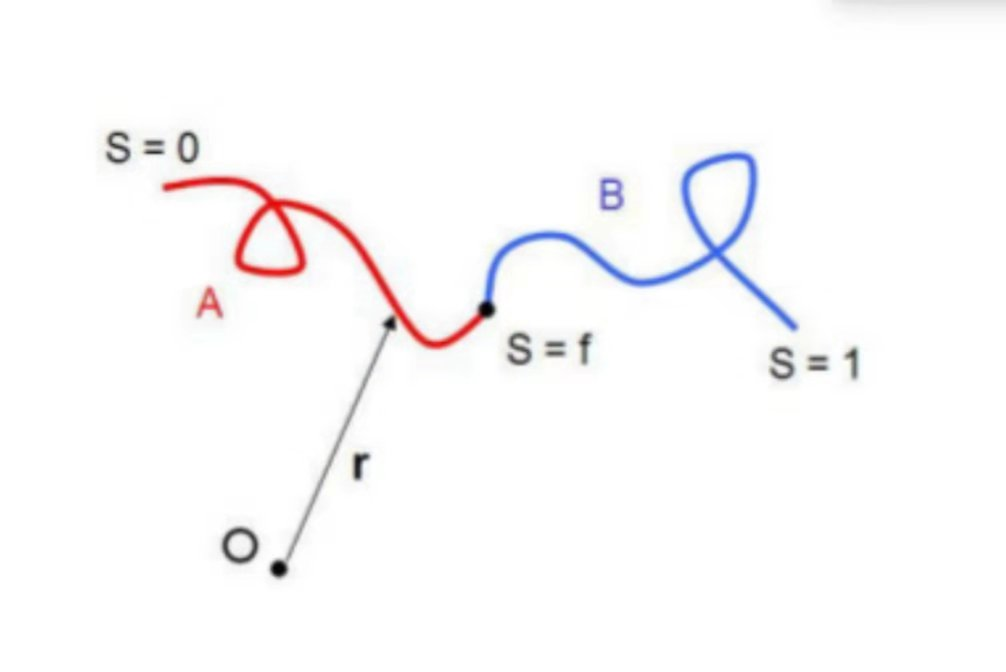
\includegraphics[width=10cm]{scft.jpg}
     \caption{两嵌段共聚物体系}
    \end{figure}
    
    该系统的哈密顿量是\\
    \begin{equation}
    H[\omega_+,\omega_-]=\frac{1}{|S|}\int dx\left\lbrace -\omega_+(x)+\frac{\omega_{-}^2(x)}{\chi N}\right\rbrace -\log Q[\omega_+(x),\omega_-(x)]	
    \end{equation}
    
    
    其中$\omega_+(x)$和$\omega_-(x)$是对应的系统的压力和对应交换化学势,$x$表示平面上的点.\\
    
    自由能函数关于场的一阶变分推导出下面的自洽场方程\\

  \begin{gather}
    \frac{\delta H}{\delta \omega_+(x)}=\phi _A(x)+\phi _B(x)-1=0 \\   
    \frac{\delta H}{\delta \omega_-(x)}=\frac{2\omega_-(x)}{\chi N}-[\phi _A(x)-\phi _B(x)]=0
   \end{gather}
   其中$\phi _A(x)$和$\phi _B(x)$是单体$A$和单体$B$的密度.再通过使用连续的高链模型,我们可以完成$SCFT$系统. 
  \begin{gather}
    Q=\frac{1}{|S|}\int dx q(x,1)=\frac{1}{|S|}\int dx q(x,s)q^{+}(x,1-s),\qquad \forall s \in[0,1]  \\
   \phi _A(x)=\frac{1}{Q}\int_0^f ds q(x,s)q^{+}(x,1-s)\\
   \phi _B(x)=\frac{1}{Q}\int_f^1 ds q(x,s)q^{+}(x,1-s)
    \end{gather}
    
    在系统中,正向传播子$q(x,s)$表示长度为$s$的链在平面位置$x$处概率权重,其中变量$s$用于参数化每条共聚物链,$s=0$表示单体$A$的起始位置,$s=f$是单体$A$和单体$B$之间的连接点.\\
    
    由柔性高斯链模型,得到正向传播子$q(x,s)$满足下面修正扩散方程\\
    
    \begin{gather}
    \frac{\partial}{\partial s}q(x,s)=\Delta q(x,s)-\omega(x,s)q(x,s),\qquad q(x,0)=1   
    \end{gather} 
      
    \begin{equation}\label{eq:dirichlet}
    \omega(x,s)=\begin{cases}
    \omega_+(x)-\omega_-(x),\qquad 0\leq s \leq f.\\
    \omega_+(x)+\omega_-(x),\qquad 1-f\leq s \leq 1 
    \end{cases}
    \end{equation}
    

    反向传播算子$q^{+}(x,s)$是由$s=1$到$s=0$的概率权重来表示.\\
    
   \begin{gather} 
   \frac{\partial}{\partial s}q^{+}(x,s)=\Delta q^{+}(x,s)-\omega^{+}(x,s)q^{+}(x,s),\qquad q^{+}(x,0)=1 \end{gather}
    \begin{equation}\label{eq:dirichlet}
    \omega^{+}(x,s)=\begin{cases}
    \omega_+(x)+\omega_-(x),\qquad 0\leq s \leq 1-f.\\
    \omega_+(x)-_\omega-(x),\qquad  Q=\frac{1}{|S|}\int dx q(x,1)=\frac{1}{|S|}\int dx q(x,s)q^{+}(x,1-s)\qquad 1-f\leq s \leq 1 
    \end{cases}
    \end{equation}
    \subsubsection{数值方法}
    
         在此采用梯度下降法达到鞍点:\\
         
    \begin{gather}    
    \frac{\partial}{\partial s}\omega_+(x,s)=\frac{\delta H[\omega_+,\omega_-]}{\delta \omega_+(x,s)}\\
    \frac{\partial}{\partial s}\omega_-(x,s)=-\frac{\delta H[\omega_+,\omega_-]}{\delta \omega_-(x,s)}    
    \end{gather}
    
    
    通过下面的迭代方法寻找SCFT的鞍点并更新$\omega_{\pm}(x)$.\\
    
    
    step1 给定初始估计的场$\omega_{\pm}(x,0)$.\\
    
    step2 计算平面上的向前(向后)传播算子$q(x,s)$和$q^+(x,s)$.\\
    
    step3 通过上述方程得到$Q$,\,$\phi_A(x)$和$\phi_B(x)$,并计算哈密顿量$H$.\\
    
    step4 对方程使用迭代方法更新场$\omega_+(x)$和$\omega_-(x)$.\\
    
    step5 重复步骤2-4,直到达到收敛标准.\\
    
  ....\\
  \subsubsection{虚单元求解自洽场模型}
  
  主要用虚单元法求解传播子方程\\
  \begin{gather}
  \frac{\partial}{\partial s}q(x,s)=\Delta q(x,s)-\omega(x,s)q(x,s),\qquad q(x,0)=1   
  \end{gather} 
  
  下面用 \.{q}(x,s)表示 $\frac{\partial}{\partial s}q(x,s)$\\
  
  上式为:\\
\begin{gather}
 \.{q}(x,s) -\Delta q(x,s)-\omega(x,s)q(x,s)=0
\end{gather}
\begin{gather}
\int\.{q}(x,s)v -\int\Delta q(x,s)v-\int\omega(x,s)q(x,s)v = 0
\end{gather}
\begin{gather}
\int\.{q}(x,s)v -\nabla q(x,s) v|_{\partial \Omega}+\int \nabla q(x,s)\nabla v-\int\omega(x,s)q(x,s)v = 0
\end{gather}




  
  
  
  
  
  
    \section{VEM的收敛}
    以谱方法求取的数值解为真解,研究虚单元方法求得的数值解的收敛情况\\
    
    可体现在三个方面:\\
    
    1. 单链配分函数Q\\
    
    2. 哈密顿量H\\
    
    3. 密度函数$\phi$ \\
    
    \subsection{谱方法spectrum method求解SCFT模型}
    
    \qquad SM方法是解偏微分方程的一种数值方法.其要点是把解近似地展开成光滑函数(一般是正交多项式)的有限级数展开式,即所谓解的近似谱展开式,再根据此展开式和原方程,求出展开式系数的方程组.一般多取切比雪夫多项式和勒让德多项式作为近似展开式的基函数.对于周期性边界条件,用傅里叶级数和面调和级数比较方便.谱方法的精度,直接取决于级数展开式的项数.\\
    
    谱方法和有限元方法密切相关, 建立在相同的思想基础上;它们之间的主要区别是, 谱方法在整个域中使用非零的基函数, 而有限元方法只在局部单元上使用非零的基函数。换句话说, 谱方法采用全局方法, 而有限元方法采用局部方法.由于这个原因, 谱方法具有很好的误差.\\
    
    在这里我们讨论一下MATLAB中FFT和IFFT与DFT的对应关系.\\
    
    首先给出:\\
    
    DFT(离散傅里叶变换):\\
    
   $$ \hat{u}=\dfrac{1}{Nc_{k}}\sum_{j=0}^{N-1}u(x_j)e^{-  ikx_j},\quad k=-N/2,\dots,N/2$$
   
   这里当$|k|< N/2$时$c_k=1$,当$k=\pm N/2$时$c_k=2$,N为偶数.\\
   
    逆离散变换:\\
  
  $$u(x_j)=\sum_{k=-N/2}^{N/2} \hat{u_k}e^{ikx_j},\quad j=0,1,\dots N$$
  
  在$\{x_k=2\pi k /N\}_{k=0}^{N-1}$给出$\{v(j)=u(x_{j-1})\}_{j=1}^{N}$\\
  
 由MATLAB命令$ \hat{v}=fft(v)$得到$\{\hat{v}(k)\}_{k=1}^N$通过\\
 
 $$\hat{v}(k)=\sum_{j=1}^{N}v(j)e^{-2\pi i(j-1)(k-1)/N},\quad 1\leq k \leq N$$
 
 iFFT可以通过Matlab命令$v=ifft(\hat  {v})$得到,返回$\{v(j)\}_{j=1}^N$通过\\
 
 $$v(j)=\dfrac{1}{N}\sum_{k=1}^{N}\hat{v}(k)e^{2\pi i(j-1(k-1)/N}, \quad 1\leq j\leq N$$
 
 令\\
 
 $$u(x_j)=v(j+1),\quad x_j=\dfrac{2\pi j}{N},\quad 0\leq j \leq N-1$$
 
 我们发现\\
 
 $$ \hat{u}_k=\dfrac{1}{N}\hat{v}(k+1), \quad 0\leq k \leq \dfrac{N}{2}-1$$
 
 $$ \hat{u}_k=\dfrac{1}{N}\hat{v}(k+N+1), \quad -\dfrac{N}{2}+1\leq k \leq-1$$
 $$ \hat{u}_{-N/2}=\hat{u}_{N/2} = \dfrac{1}{2N}\hat{v}(N/2+1)$$
 
 整理得到下表:\\
 
\begin{table}[H]
	\centering
	\begin{tabular}{ccccccccccc}
		
		\toprule
		j&1& 2  &$\dots$&N/2-1&N/2&N/2+1&N/2+2&$\dots$&N-1&N\\
		\midrule    
       $u=v$&$u_0$&$u_1$&$\dots$&$\dots$&$\dots$&$\dots$&$\dots$&$\dots$&$u_{N-2}$&$u_{N-1}$\\
       $\hat{u}=\hat{v}/N$&$\hat{u}_0$&$\hat{u}_1$&$\dots$&$\hat{u}_{N/2-2}$&$2\hat{u}_{N/2-1}$&$\hat{u}_{N/2}$&$\hat{u}_{-N/2+1}$&$\dots$&$\hat{u}_{-2}$&$\hat{u}_{-1}$\\
       k&0&1&$\dots$&N/2-2&N/2-1&-N/2&-N/2+1&$\dots$&-2&-1\\
		\bottomrule
	\end{tabular}
\end{table} 

表中最后一行为FFT中\textbf{k}的取值.\\
	 

    谱方法的思路:对PDE方程进行FFT变换,得到只对时间微分的常微分方程组.然后,利用时间离散来解ODE方程组.\\
    
    算子分裂法:解微分方程的一种数值方法.在一个时间步长里,将原始方程分离成两部分来分别求解,然后将两部分的解合并形成原方程的解.\\
    
    具体求解过程:\\
    
    周期边界条件\\
   
    空间:谱方法\\
  
    时间:算子分裂法 \\
    
    1.给出初值$\omega_-(x)$.\\
    
    2.求解$q(x,s)$和$q^+(x,s)$\\
     \begin{gather}
    \frac{\partial}{\partial s}q(x,s)=\Delta q(x,s)-\omega(x,s)q(x,s)  :=\mathcal{L}_1(q)+ \mathcal{L}_2(q) 
    \end{gather}
    \textbf{step1}:(半步,即时间$s=\dfrac{\tau}{2}$)$\tau$为时间步长.\\
    
    求解$$\frac{\partial}{\partial s}q(x,s)=\Delta q(x,s):=\mathcal{L}_1(q)$$\\
    
    
     利用傅里叶变换有: $$q(x,s)= \sum_{k} \hat{q}(k,s)e^{ikx}$$\\
     
     $$\frac{\partial}{\partial s} \sum_{k}\hat{q}(k,s)e^{ikx} =\Delta\sum_{k}\hat{q} (k,s)e^{ikx}=\sum_{k}-k^2\hat{q}(k,s)e^{ikx}$$\\
     
     两边同时与$e^{-ijx}$做内积,当$j=k$时,$\langle e^{-ikx},e^{-ijx}\rangle=1$;当$j \neq k$时,$\langle e^{-ikx},e^{-ijx}\rangle=0.$\\
     
     故化简方程为:\\
     $$\frac{d\hat{q}(k,s)}{ds} = -k^2\hat{q}(k,s)$$
     $$ \frac{d\hat{q}(k,s)}{\hat{q}(k,s)} = -k^2ds $$
     $$\hat{q}(k,s)=e^{-k^2s+c}=e^{-k^2s}e^{c} $$
     
     当$s=0$时,$\hat{q}(k,0)= e^{c} $\\
     
     故:
     $$\hat{q}(k,s)=e^{-k^2s}\hat{q}(k,0)$$
     \textbf{step2}:(一步,即时间$s=\tau$)\\
     
     求解$$\frac{\partial}{\partial s}q(x,s)=-\omega(x,s)q(x,s)  :=\mathcal{L}_2(q)$$
     $$\dfrac{q(x,s)}{ds}=-\omega(x,s)q(x,s)$$
     $$\dfrac{q(x,s)}{q(x,s)}=-\omega(x,s)ds$$
     $$q(x,s)=e^{-\omega(x,s)s}e^c$$
     当$s=0$时,$q(x,0)= e^{c} $\\
     故:
     $$q(x,s)=e^{-\omega(x,s)s}q(x,0)$$
     
     注:这里的$q(x,0)$为\textbf{step1}最终得到的$q(x,s)$.\\ 
     \textbf{step3}:(半步)重复第一步\\
     
      注:这里的$q(x,0)$为\textbf{step2}最终得到的$q(x,s)$.\\
      
    \textbf{step1}--复\\
    
    \textbf{step2}--实\\
    
    \textbf{step3}--复\\
     
     同理求得$q^+(x,s)$.\\
     
     3.计算Q和$\phi_A$和$\phi_B$\\
     
      $$Q=\frac{1}{|S|}\int dx q(x,s)q^{+}(x,1-s)
      \overset{s=1}{=}\frac{1}{|S|}\int dx q(x,1)$$
      
      $$\int q(x,1) dx=\int\sum_{k}\hat{q}(k,1)e^{-ikx}dx=\sum_{k}\hat{q}(k,1)\int e^{-ikx}e^{-i0x}dx=\hat{q}(0,1)$$
      
      
     得到:$Q=\hat{q}(0,1)$\\
     
      $$\phi _A(x)=\frac{1}{Q}\int_0^f ds q(x,s)q^{+}(x,1-s)$$
      $$\phi _B(x)=\frac{1}{Q}\int_f^1 ds q(x,s)q^{+}(x,1-s)$$
      
      采用四阶离散格式:\\
      
      $$\int_{0}^{n_s}=\tau \{-\frac{5}{8}(f_0+f_{n_s})+\frac{1}{6}(f_1+f_{n_s-1})-\frac{1}{24}(f_2+f_{n_s-2})+\sum_{j=0}^{n_s}f_j\}$$
      
     可得$\phi_A$和$\phi_B$.\\
     
     4.更新场函数\\
     
     \begin{gather}    
     \frac{\partial}{\partial s}\omega_+(x,s)=\frac{\delta H[\omega_+,\omega_-]}{\delta \omega_+(x,s)}=\phi _A(x)+\phi _B(x)-1\\
     \frac{\partial}{\partial s}\omega_-(x,s)=-\frac{\delta H[\omega_+,\omega_-]}{\delta \omega_-(x,s)}=\phi _A(x)-\phi _B(x)-\frac{2\omega_-(x,s)}{\chi N} 
     \end{gather}
     用向前欧拉迭代:\\
     
     $$\frac{\partial}{\partial s}\omega_+(x,s^n)=\dfrac{\omega_+(x,s^{n+1})-\omega_+(x,s^{n})}{\Delta s}$$
     故$\omega_+(x,s)$迭代公式为:\\
     $$\omega_+(x,s^{n+1})=\omega_+(x,s^n)+\Delta s[{\phi _A}^n(x)+{\phi _B}^n(x)-1]$$
     
     同理:\\
     
     $\omega_-(x,s)$迭代公式为:\\
     $$\omega_-(x,s^{n+1}=\omega_-(x,s^n)+\Delta s[{\phi _A}^n(x)-{\phi _B}^n(x)-\frac{2\omega_-(x,s^n)}{\chi N}]$$
     5.重复迭代,直到达到收敛标准$1.0e-6$,得到结果.\\
     
    当N=8,即空间剖分为8*8网格时,$\phi$ 的值为:
    \begin{table}[H]
    	\centering
    	\begin{tabular}{ccccccccc}
    		
    		\toprule
    		N&1& 2  &3&4&5&6&7&8\\
    		\midrule    
    		1&0.1947&	0.2062&	0.1937&	0.2057&	0.1951&	0.2040&	0.1964&	0.2040\\
    		2&0.2021&	0.1970&	0.2029&	0.1974&	0.2018&	0.1988&	0.2007&	0.1988\\
    		3&0.1993&	0.2011&	0.1988&	0.2008&	0.1996&	0.1998&	0.2005&	0.1997\\
    		4&0.2018&	0.1976&	0.2023&	0.1979&	0.2016&	0.1988&	0.2007&	0.1989\\
    		5&0.1981&	0.2023&	0.1976&	0.2020&	0.1983&	0.2011&	0.1991&	0.2010\\
    		6&0.2006&	0.1988&	0.2011&	0.1991&	0.2003&	0.2002&	0.1994&	0.2002\\
    		7&0.1974&	0.2031&	0.1967 &	0.2027&	0.1978&	0.2014&	0.1989&	0.2014\\
    		8&0.2054&	0.1937&	0.2063&	0.1941&	0.2049&	0.1959&	0.2036&	0.1958\\
    		\bottomrule
    	\end{tabular}
    \end{table} 
    当N=128,即空间剖分为128*128网格时,相结构为:\\
    \begin{figure}[H] 
    	\centering
    	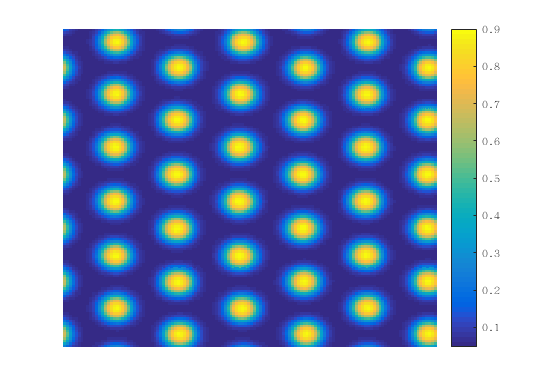
\includegraphics[width=10cm]{p.png}
    \end{figure}
    相同网格下,VEM得到的结果为:\\
    \begin{figure}[H] 
    	\centering
    	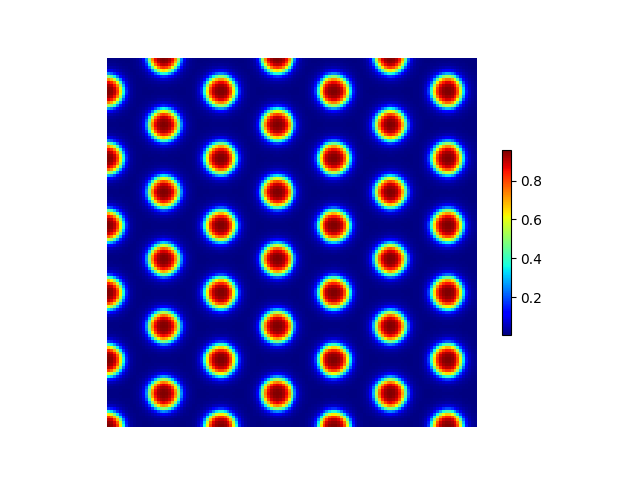
\includegraphics[width=10cm]{scftfigure5770.png}
    \end{figure}         
     
     
     
     
     
    
    
    
    
    \subsection{过程中所遇到的困难}
    
    校验谱方法数值解的正确,如下:\\
    
    $dt=0.1$\\
     \begin{table}[H]
     	\centering
     	\begin{tabular}{ccc}
     		
     		\toprule
     		N&Q & H \\
     		\midrule    
     		128&91.090613&-2.2510955\\
     		256&91.070881&-2.2510601\\
     		512&91.062020&-2.2510440\\
     		\bottomrule
     	\end{tabular}
     \end{table} 
    
     
    
    当虚单元方法中的网格结构为方形,即:\\
        \begin{figure}[H] 
        	\centering
        	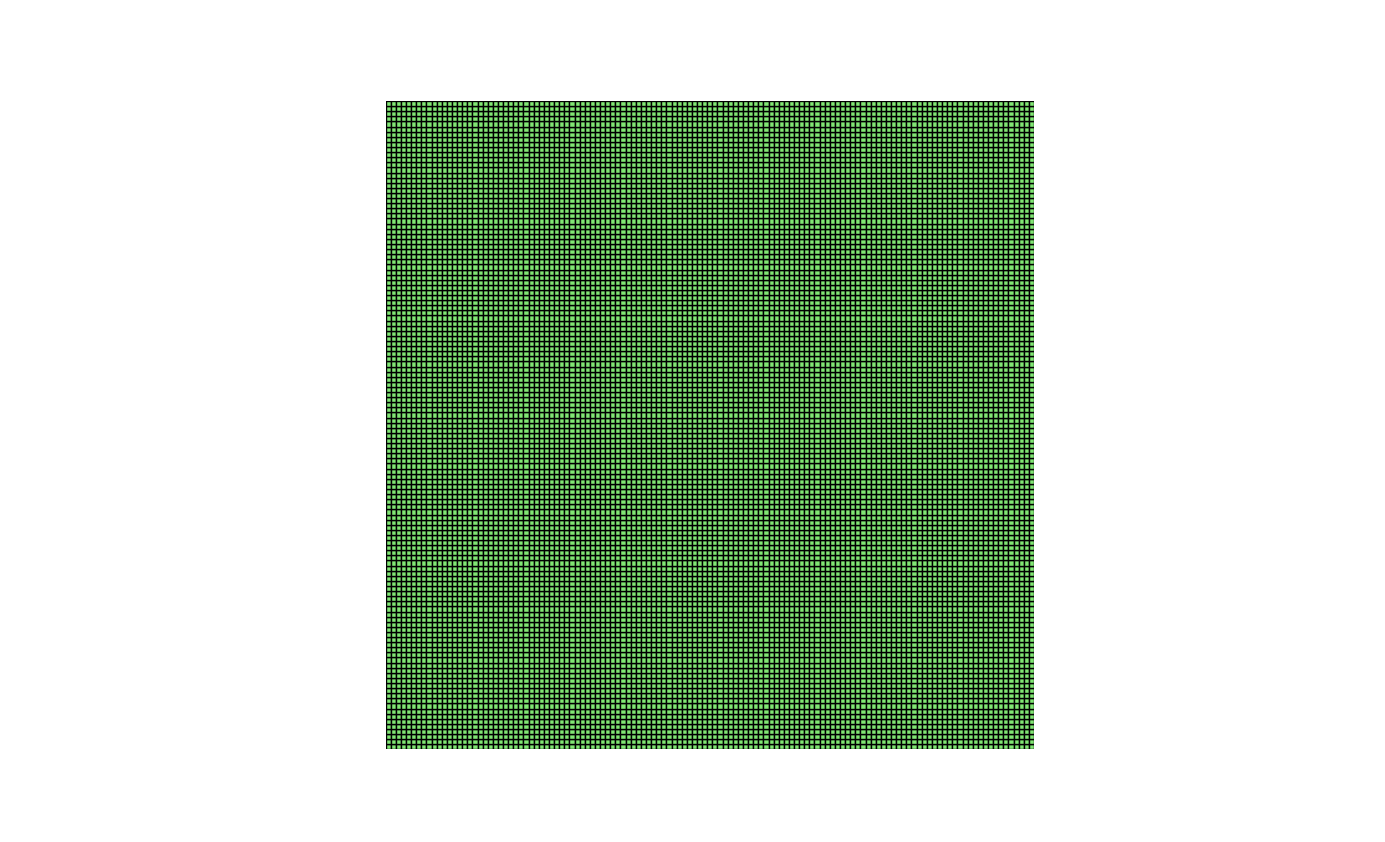
\includegraphics[width=10cm]{vem.png}
        	\caption{网格结构}
        \end{figure}
        网格为128*128\\
        
    初值取六状:\\
    
        $ \mu_+=0 $\\
        
        $ \mu_-=\cos^{2}x+\cos^2 (\frac{x}{2}+\frac{\sqrt{3}y}{2})+\cos^2(-\frac{x}{2}+\frac{\sqrt{3}y}{2})+\cos^{2}(-x)+\cos^2 (-\frac{x}{2}-\frac{\sqrt{3}y}{2})+\cos^2 (\frac{x}{2}-\frac{\sqrt{3}y}{2})$\\
        
        初值结果为:\\
             \begin{table}[H]
             	\centering
             	\begin{tabular}{ccc}
             		
             		\toprule
             		&谱方法 & VEM  \\
             		\midrule    
             		Q&6.668754e-02&6.660827e-02\\
             		H&3.069368e+00&4.096418e+00\\
             		\bottomrule
             	\end{tabular}
             \end{table} 
             最终结果为:\\
             
$dt=0.005$\\             
 \begin{table}[H]
 	\centering
 	\begin{tabular}{cccccc}
 		
 		\toprule
 	 &  \multicolumn{4}{c}{VEM}	&\multirow{3}*{谱方法} \\
 		\cmidrule(lr){2-5}
 		&  N=64& N=128&N=150&N=200\\
 		\midrule    
 		Q&293.600689&375.240925&382.029489&390.319270&397.473100\\
 		H&-2.364668&-2.377752&-2.378390&-2.379013&-2.377445\\
 		\bottomrule
 	\end{tabular}
 \end{table} 
    
   \section{数值模拟}

    
    节点$x=(x,y)$\\
    
    六状相\\
    
    初值:\\
    
    $ \mu_+=0 $\\
    
    $ \mu_-=\cos^{2}x+\cos^2 (\frac{x}{2}+\frac{\sqrt{3}y}{2})+\cos^2(-\frac{x}{2}+\frac{\sqrt{3}y}{2})+\cos^{2}(-x)+\cos^2 (-\frac{x}{2}-\frac{\sqrt{3}y}{2})+\cos^2 (\frac{x}{2}-\frac{\sqrt{3}y}{2})$\\
   
    参数:\\
    
     $f_A=0.2,\chi_N=25,tol=1.0e-6$\\
     
     层状相\\
     
     初值:\\
    
    $ \mu_+=0 $\\
    
    $ \mu_-=sin(4*x)$\\

    参数:\\
    
     $f_A=0.5,\chi_N=15,tol=1.0e-6$\\
     \subsection{方形区域}
   
     \begin{table}[H]
     	\centering
     	    \begin{tabular}{cccc}
     	    	
     	    	\toprule
     	    	区域$D/cm^2$&迭代步数 & Q &  H \\
     	    	\midrule    20*20(六状)&213&3.754509448730350e+02&-2.377792466775116e+00\\
     	    	20*20(层状)&272& 5.221890824944924e+00 &-3.041094000606217e-01\\
     	    	\bottomrule
     	    \end{tabular}
     \end{table} 

    
\begin{figure}[H]
	% 调整字体和图片间距;
	\setlength{\abovecaptionskip}{0.cm}
	\setlength{\belowcaptionskip}{-0.cm}
	% 插入子图;
	\begin{minipage}[!htbp]{0.3\linewidth}
		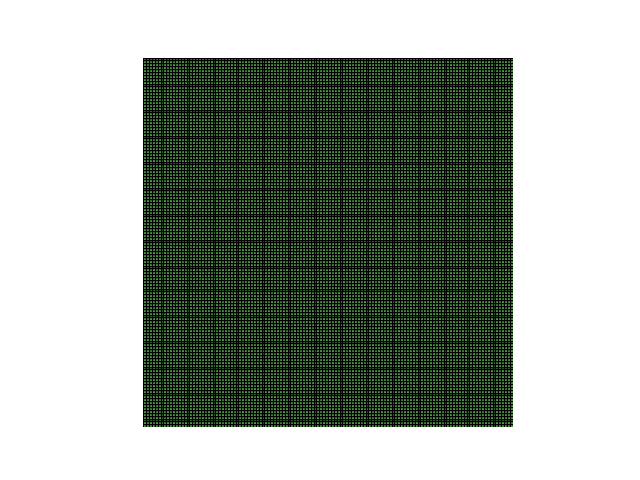
\includegraphics[width=5.2cm]{22.png}
		\caption*{网格结构}
	\end{minipage}
	\hspace{0.23in}
	\begin{minipage}[!htbp]{0.3\linewidth}
		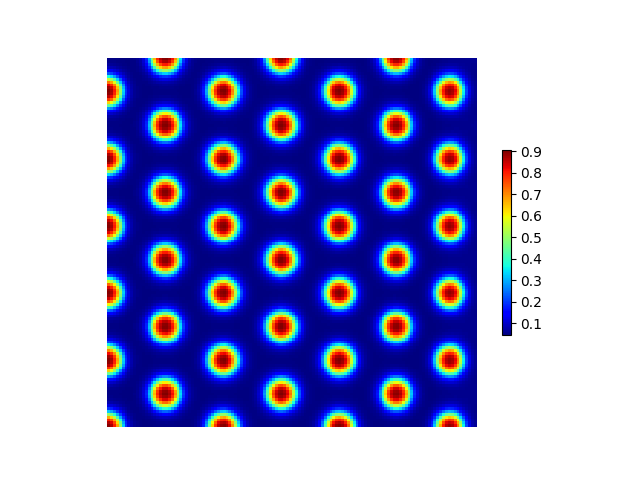
\includegraphics[width=5.2cm]{scftfigure200.png}
		\caption*{六状相}
	\end{minipage}
	\hspace{0.23in}
	\begin{minipage}[!htbp]{0.3\linewidth}
		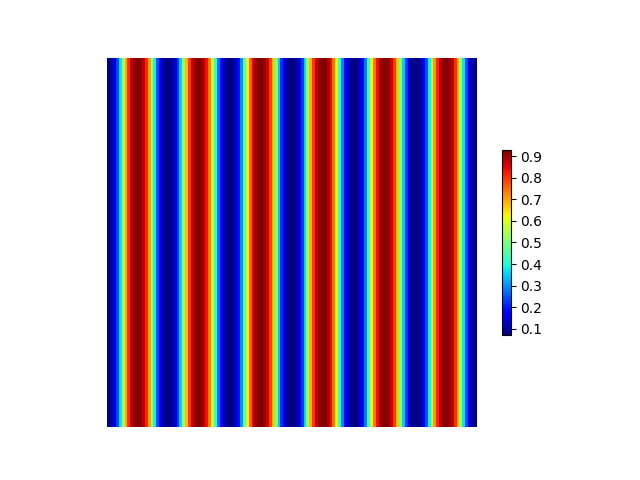
\includegraphics[width=5.2cm]{scftfigure240.png}
		\caption*{层状相}
	\end{minipage}	
\end{figure}
      
 \subsection{有三个洞的方形区域}   
    \begin{table}[H]
    		\centering
    	\begin{tabular}{cccc}
    		\toprule
    		区域$D/cm^2$ &	迭代步数 & Q &  H \\
    		\midrule
    		21*17.5(六状)&660 &2.345568135858854e+02&-2.372255051066200e+00\\
    				21*17.5(层状)&640& 5.187955000344139e+00 & -3.049841420411299e-01\\
    		\bottomrule
    	\end{tabular}
    \end{table}
      
\begin{figure}[H]
 % 调整字体和图片间距;
 \setlength{\abovecaptionskip}{0.cm}
 \setlength{\belowcaptionskip}{-0.cm}
 % 插入子图;
 \begin{minipage}[!htbp]{0.3\linewidth}
 	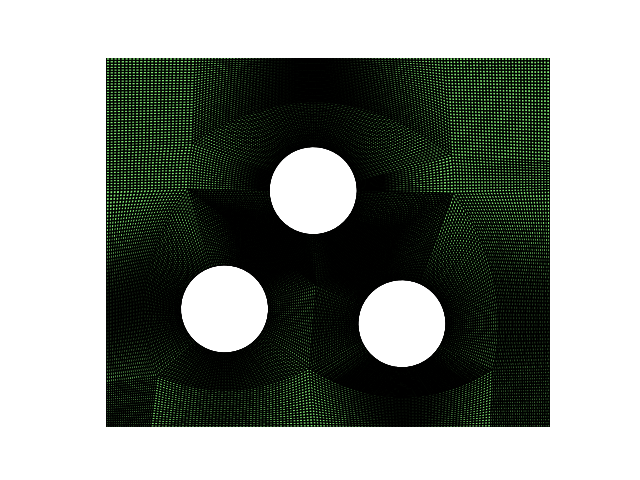
\includegraphics[width=5.2cm]{Figure_11.png}
 	\caption*{网格结构}
 \end{minipage}
 \hspace{0.23in}
 \begin{minipage}[!htbp]{0.3\linewidth}
 	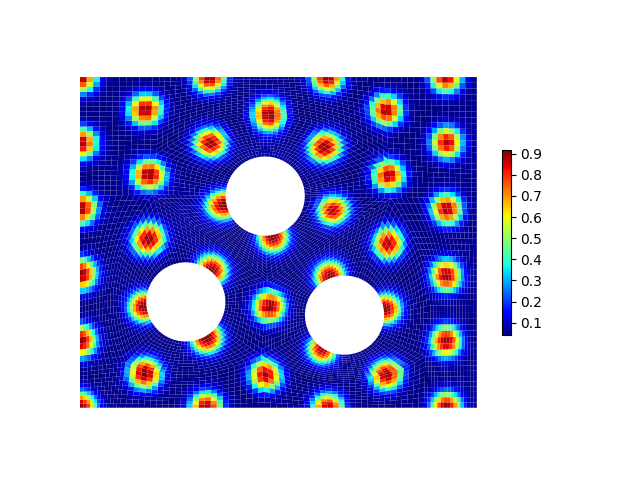
\includegraphics[width=5.2cm]{scftfigure640.png}
 	\caption*{六状相}
 \end{minipage}
 	\hspace{0.23in}
 	\begin{minipage}[!htbp]{0.3\linewidth}
 		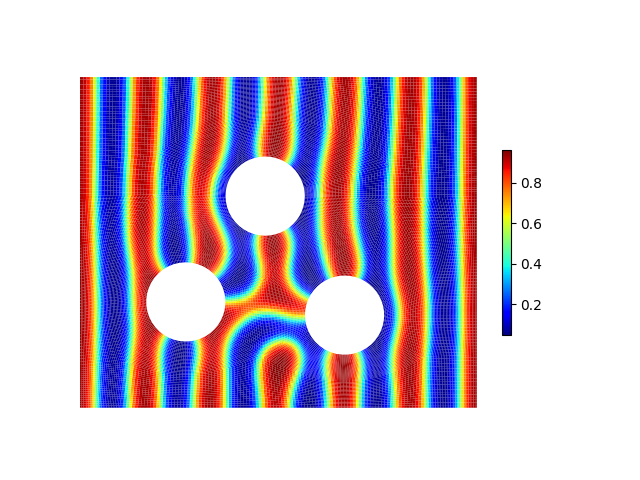
\includegraphics[width=5.2cm]{scftfigure.png}
 		\caption*{层状相}
 	\end{minipage}
 \end{figure}     

\subsection{花瓣型区域}   
      \begin{table}[H]
      		\centering
      	\begin{tabular}{cccc}
      		\toprule
      		区域$D/cm^2$ &	迭代步数 & Q &  H \\
      		\midrule
      		20*20(六状)&586& 3.202963848832981e+02 & -2.374249956123630e+00\\
      		20*20(层状)&1740 &1.009842899971281e+02 & -1.738873865311719e+00\\
      		\bottomrule
      	\end{tabular}
      \end{table}
      
      \begin{figure}[H]
      	% 调整字体和图片间距;
      	\setlength{\abovecaptionskip}{0.cm}
      	\setlength{\belowcaptionskip}{-0.cm}
      	% 插入子图;
      	\begin{minipage}[!htbp]{0.3\linewidth}
      		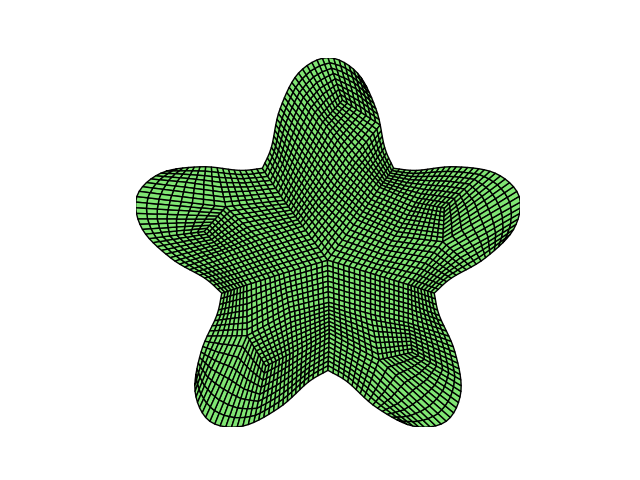
\includegraphics[width=5.2cm]{Figure_hc.png}
      		\caption*{网格结构}
      	\end{minipage}
      	\hspace{0.23in}
      	\begin{minipage}[!htbp]{0.3\linewidth}
      		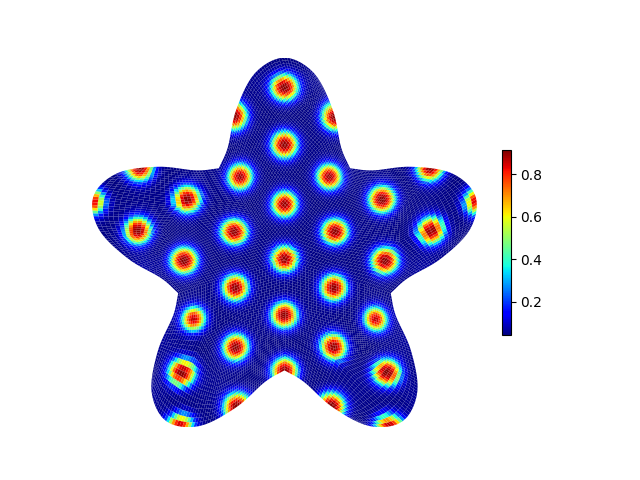
\includegraphics[width=5.2cm]{scftfigure584.png}
      		\caption*{六状相}
      	\end{minipage}
      	\hspace{0.23in}
      	\begin{minipage}[!htbp]{0.3\linewidth}
      		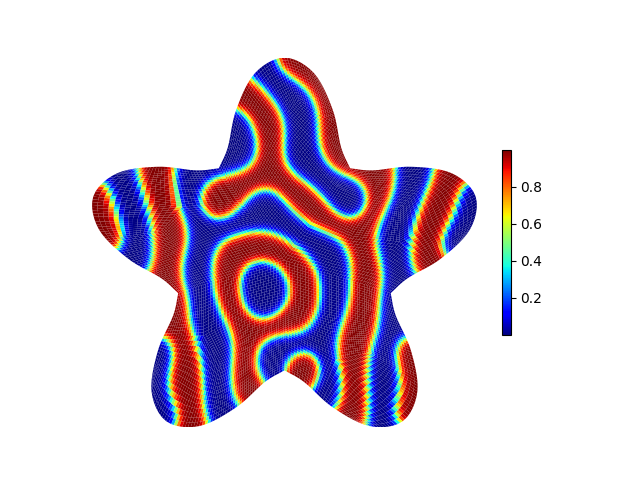
\includegraphics[width=5.2cm]{scftfigure1740.png}
      		\caption*{层状相}
      	\end{minipage}
      \end{figure} 
    
  \subsection{L型区域}   
  \begin{table}[H]
  		\centering
  	\begin{tabular}{cccc}
  		\toprule
  		区域$D/cm^2$ &	迭代步数 & Q &  H \\
  		\midrule
  		20*20(六状)&9479 &1.535787456514685e+00 & -2.276253333369957e+00\\
  		20*20(层状)&404& 4.063629265390633e+01 & -1.639327262484907e+00\\
  		\bottomrule
  	\end{tabular}
  \end{table}
  
  \begin{figure}[H]
  	% 调整字体和图片间距;
  	\setlength{\abovecaptionskip}{0.cm}
  	\setlength{\belowcaptionskip}{-0.cm}
  	% 插入子图;
  	\begin{minipage}[!htbp]{0.3\linewidth}
  		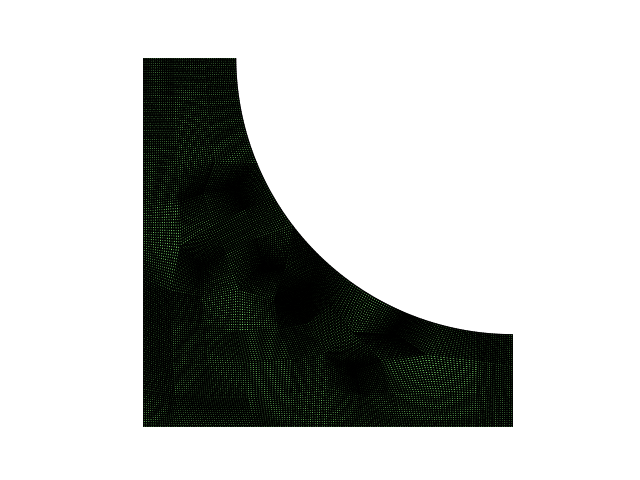
\includegraphics[width=5.2cm]{Figure_Lc.png}
  		\caption*{网格结构}
  	\end{minipage}
  	\hspace{0.23in}
  	\begin{minipage}[!htbp]{0.3\linewidth}
  		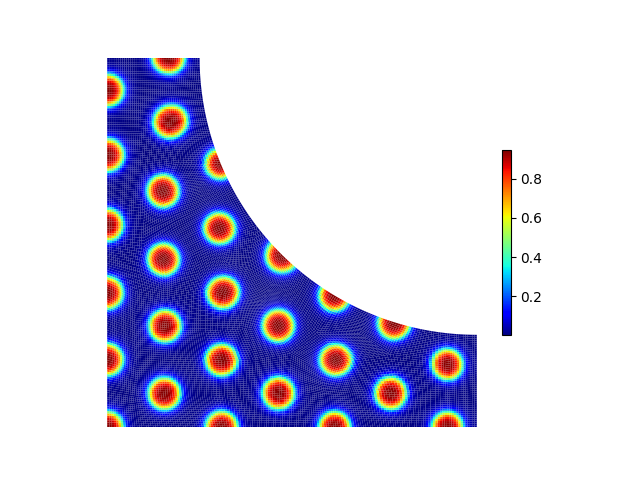
\includegraphics[width=5.2cm]{scftfigure9480.png}
  		\caption*{六状相}
  	\end{minipage}
  	\hspace{0.23in}
  	\begin{minipage}[!htbp]{0.3\linewidth}
  		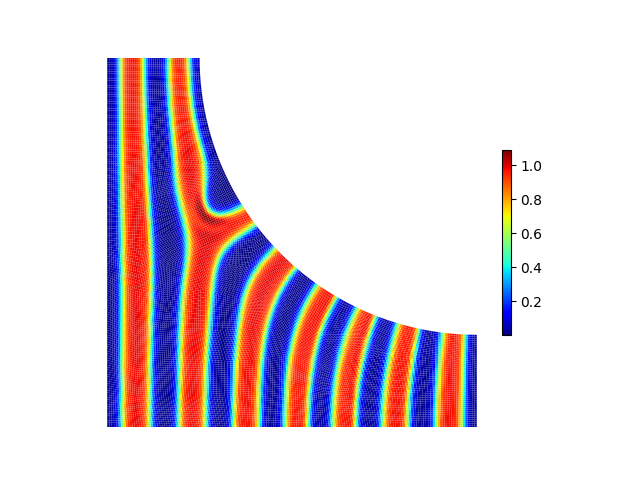
\includegraphics[width=5.2cm]{scftfigure400.png}
  		\caption*{层状相}
  	\end{minipage}
  \end{figure}
  \subsection{不规则区域}   
  \begin{table}[H]
  		\centering
  	\begin{tabular}{cccc}
  		\toprule
  		区域$D/cm^2$ &	迭代步数 & Q &  H \\
  		\midrule
  		30*22.5(六状)&212& 9.723117073842296e+02 & -2.906410995536519e+00\\
  		30*22.5(层状)&899 &1.175466270804054e+00 & -1.723618193342877e+00\\
  		\bottomrule
  	\end{tabular}
  \end{table}
  
  \begin{figure}[H]
  	% 调整字体和图片间距;
  	\setlength{\abovecaptionskip}{0.cm}
  	\setlength{\belowcaptionskip}{-0.cm}
  	% 插入子图;
  	\begin{minipage}[!htbp]{0.3\linewidth}
  		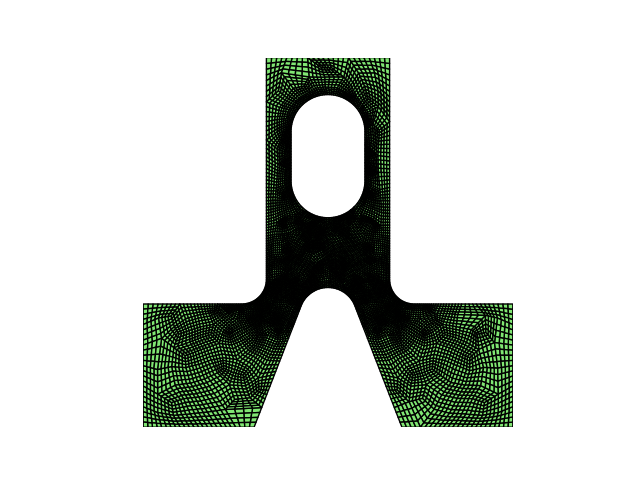
\includegraphics[width=5.2cm]{Figure_bc.png}
  		\caption*{网格结构}
  	\end{minipage}
  	\hspace{0.23in}
  	\begin{minipage}[!htbp]{0.3\linewidth}
  		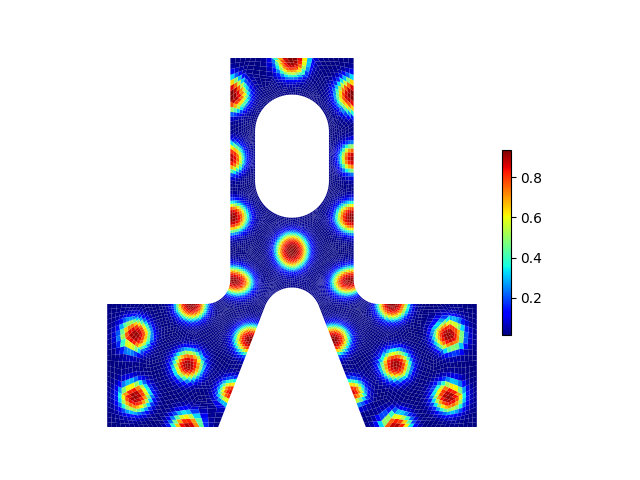
\includegraphics[width=5.2cm]{scftfigurebuming.png}
  		\caption*{六状相}
  	\end{minipage}
  	\hspace{0.23in}
  	\begin{minipage}[!htbp]{0.3\linewidth}
  		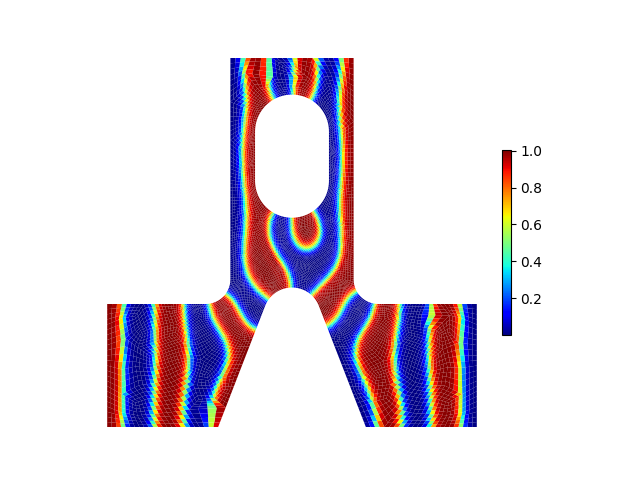
\includegraphics[width=5.2cm]{scftfigure880.png}
  		\caption*{层状相}
  	\end{minipage}
  \end{figure}
    \subsection{凹型区域}   
    \begin{table}[H]
    		\centering
    	\begin{tabular}{cccc}
    		\toprule
    		区域$D/cm^2$ &	迭代步数 & Q &  H \\
    		\midrule
    		40*24(六状)&4011 &3.649879647033268e-01 & -2.249952383796924e+00\\
    		40*24(层状)&81& 1.837812303724294e+01 & -1.012557461621539e+00\\
    		\bottomrule
    	\end{tabular}
    \end{table}
    
    \begin{figure}[H]
    	% 调整字体和图片间距;
    	\setlength{\abovecaptionskip}{0.cm}
    	\setlength{\belowcaptionskip}{-0.cm}
    	% 插入子图;
    	\begin{minipage}[!htbp]{0.3\linewidth}
    		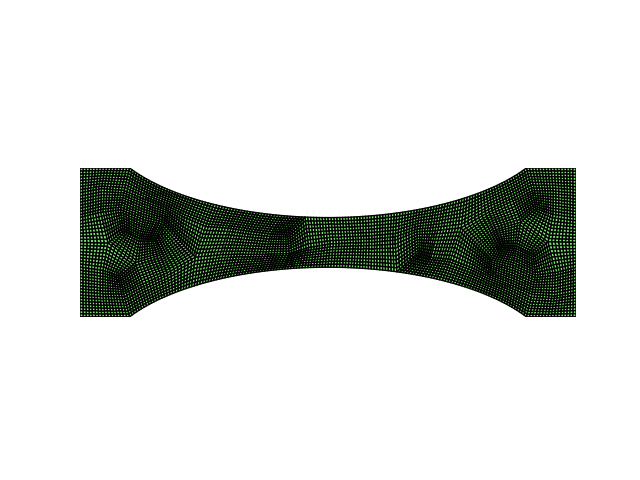
\includegraphics[width=5.2cm]{Figure_ac.png}
    		\caption*{网格结构}
    	\end{minipage}
    	\hspace{0.23in}
    	\begin{minipage}[!htbp]{0.3\linewidth}
    		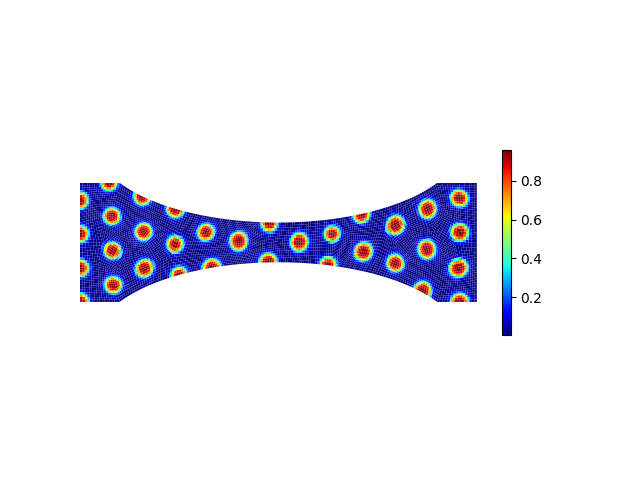
\includegraphics[width=5.2cm]{scftfigure4000.png}
    		\caption*{六状相}
    	\end{minipage}
    	\hspace{0.23in}
    	\begin{minipage}[!htbp]{0.3\linewidth}
    		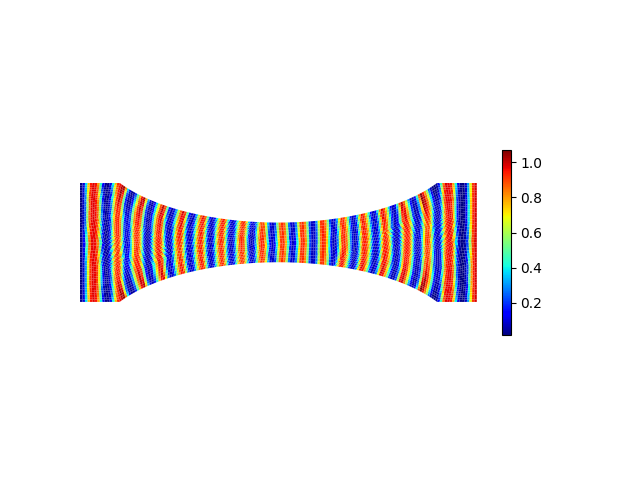
\includegraphics[width=5.2cm]{scftfigure80.png}
    		\caption*{层状相}
    	\end{minipage}
    \end{figure} 
    \subsection{机翼型区域}   
    \begin{table}[H]
    		\centering
    	\begin{tabular}{cccc}
    		\toprule
    		区域$D/cm^2$ &	迭代步数 & Q &  H \\
    		\midrule
    		70*7(六状)&6724 &3.486261454912840e-01 & -2.250387578159935e+00\\
    		70*7(层状)&260 &2.514889756039829e+02& -2.123028505807197e+00\\
    		\bottomrule
    	\end{tabular}
    \end{table}
    
    \begin{figure}[H]
    	% 调整字体和图片间距;
    	\setlength{\abovecaptionskip}{0.cm}
    	\setlength{\belowcaptionskip}{-0.cm}
    	% 插入子图;
    	\begin{minipage}[!htbp]{0.3\linewidth}
    		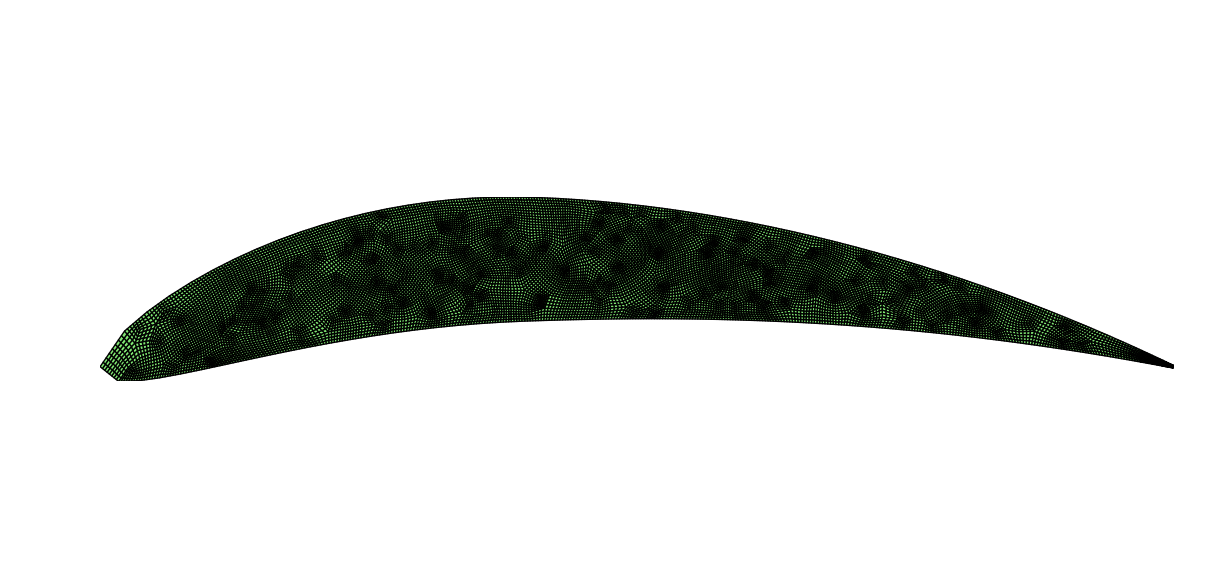
\includegraphics[width=5.2cm]{air_c.png}
    		\caption*{网格结构}
    	\end{minipage}
    	\hspace{0.23in}
    	\begin{minipage}[!htbp]{0.3\linewidth}
    		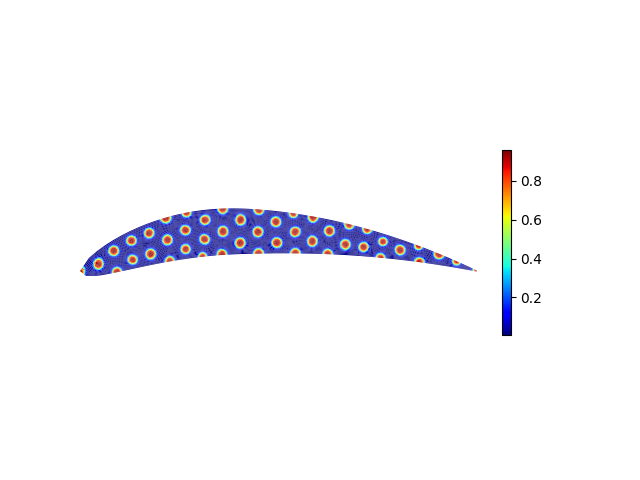
\includegraphics[width=5.2cm]{scftfigure6720.png}
    		\caption*{六状相}
    	\end{minipage}
    	\hspace{0.23in}
    	\begin{minipage}[!htbp]{0.3\linewidth}
    		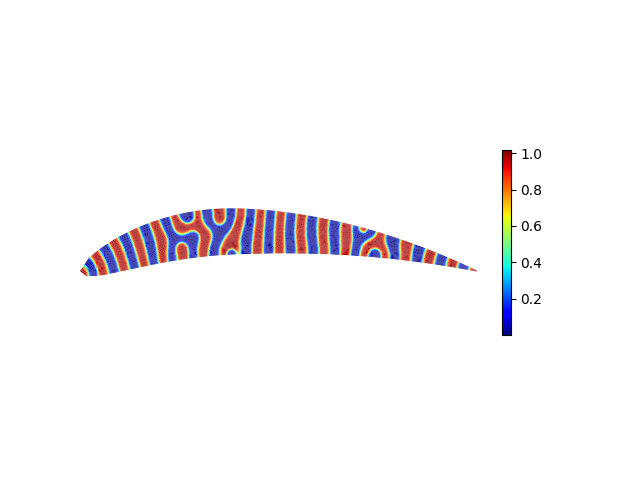
\includegraphics[width=5.2cm]{scftfigure260.png}
    		\caption*{层状相}
    	\end{minipage}
    \end{figure} 


   \section{多边形结构数值模拟}


节点$x=(x,y)$\\

六状相\\

初值:\\

$ \mu_+=0 $\\

$ \mu_-=\cos^{2}x+\cos^2 (\frac{x}{2}+\frac{\sqrt{3}y}{2})+\cos^2(-\frac{x}{2}+\frac{\sqrt{3}y}{2})+\cos^{2}(-x)+\cos^2 (-\frac{x}{2}-\frac{\sqrt{3}y}{2})+\cos^2 (\frac{x}{2}-\frac{\sqrt{3}y}{2})$\\

参数:\\

$f_A=0.2,\chi_N=25,tol=1.0e-6$\\

层状相\\

初值:\\

$ \mu_+=0 $\\

$ \mu_-=sin(4*x)$\\

参数:\\

$f_A=0.5,\chi_N=15,tol=1.0e-6$\\ 

\subsection{花瓣型区域}   
\begin{table}[H]
	\centering
	\begin{tabular}{cccc}
		\toprule
		区域$D/cm^2$ &	迭代步数 & Q &  H \\
		\midrule
		20*20(六状)&626& 3.490319185439354e+02 & -2.375424510474807e+00\\
		20*20(层状)&1395 &2.753715279880133e+01 &-1.793820469496744e+00\\
		\bottomrule
	\end{tabular}
\end{table}

\begin{figure}[H]
	% 调整字体和图片间距;
	\setlength{\abovecaptionskip}{0.cm}
	\setlength{\belowcaptionskip}{-0.cm}
	% 插入子图;
	\begin{minipage}[!htbp]{0.3\linewidth}
		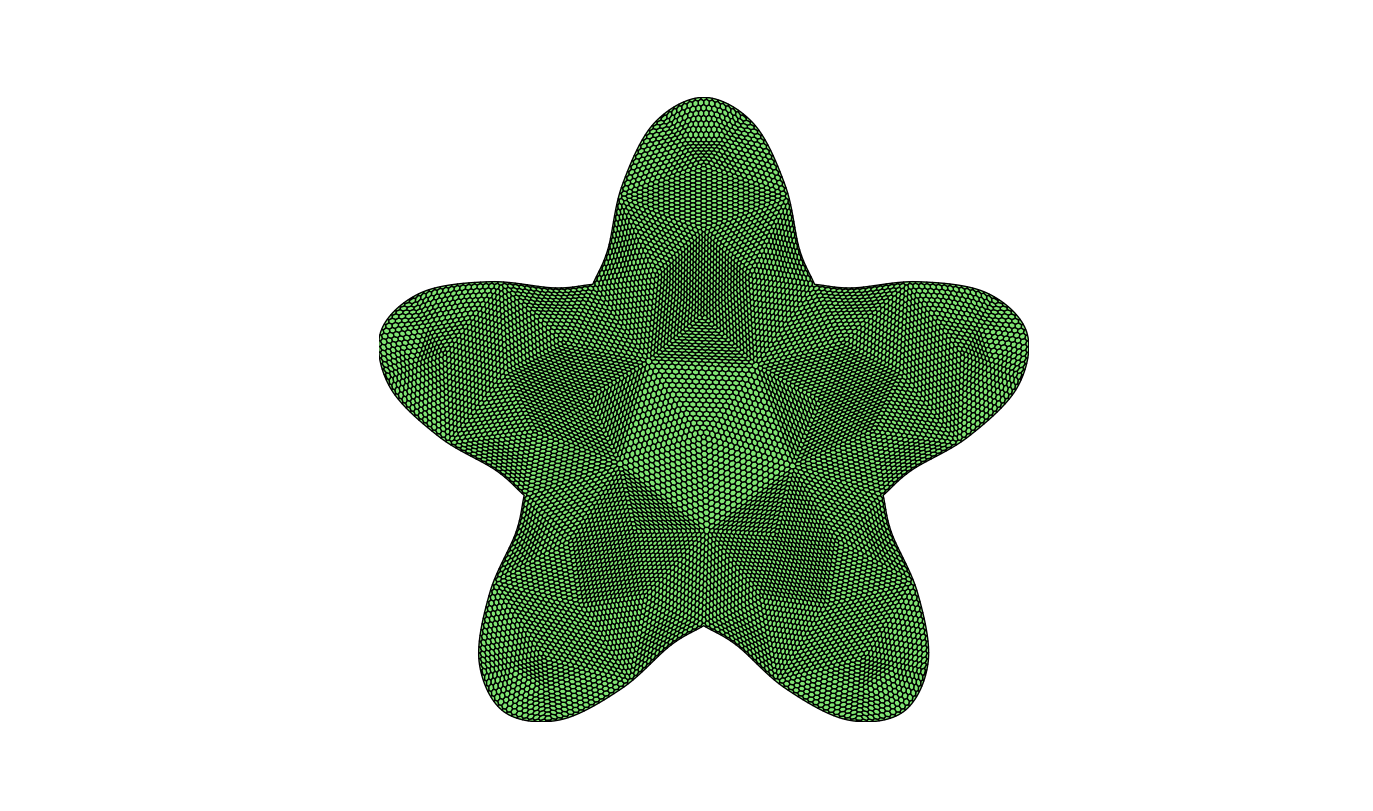
\includegraphics[width=5.2cm]{Figure_huaban.png}
		\caption*{网格结构}
	\end{minipage}
	\hspace{0.23in}
	\begin{minipage}[!htbp]{0.3\linewidth}
		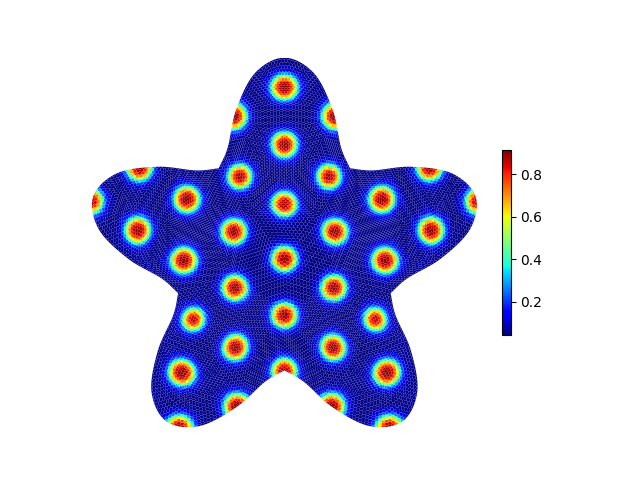
\includegraphics[width=5.2cm]{scftfigure626.png}
		\caption*{六状相}
	\end{minipage}
	\hspace{0.23in}
	\begin{minipage}[!htbp]{0.3\linewidth}
		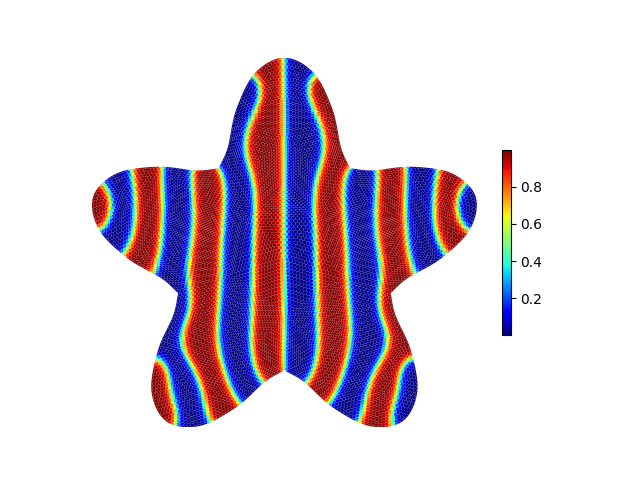
\includegraphics[width=5.2cm]{scftfigure1394.png}
		\caption*{层状相}
	\end{minipage}
\end{figure} 

\subsection{L型区域}   
\begin{table}[H]
	\centering
	\begin{tabular}{cccc}
		\toprule
		区域$D/cm^2$ &	迭代步数 & Q &  H \\
		\midrule
		20*20(六状)&313 &3.489595347550497e+02 &-2.376593651193064e+00\\
		20*20(层状)&1004 &7.199195813427511e+00 &-1.738203246649924e+00\\
		\bottomrule
	\end{tabular}
\end{table}

\begin{figure}[H]
	% 调整字体和图片间距;
	\setlength{\abovecaptionskip}{0.cm}
	\setlength{\belowcaptionskip}{-0.cm}
	% 插入子图;
	\begin{minipage}[!htbp]{0.3\linewidth}
		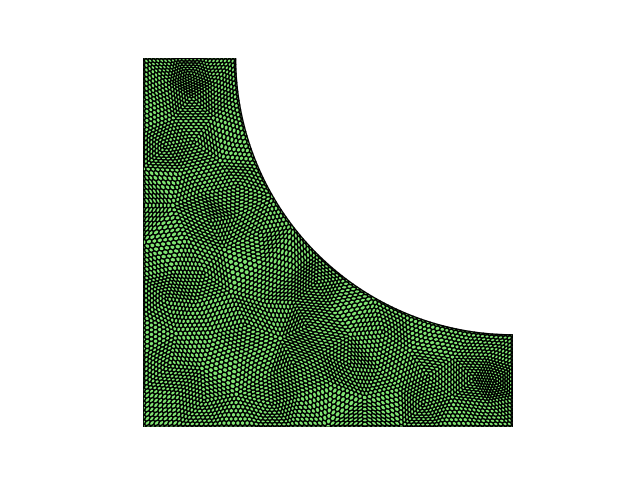
\includegraphics[width=5.2cm]{Figure_L.png}
		\caption*{网格结构}
	\end{minipage}
	\hspace{0.23in}
	\begin{minipage}[!htbp]{0.3\linewidth}
		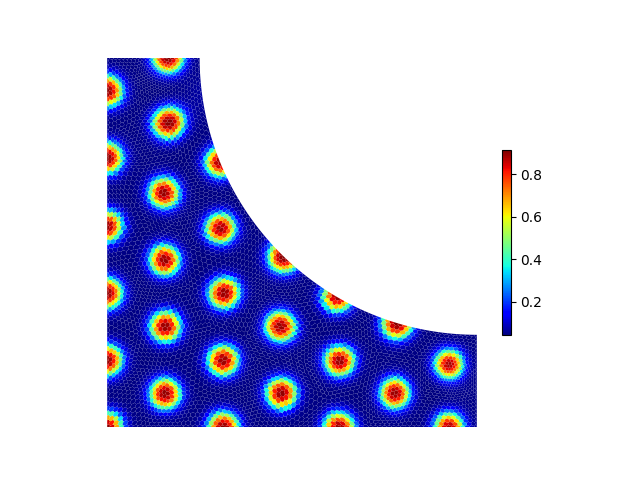
\includegraphics[width=5.2cm]{scftfigure312.png}
		\caption*{六状相}
	\end{minipage}
	\hspace{0.23in}
	\begin{minipage}[!htbp]{0.3\linewidth}
		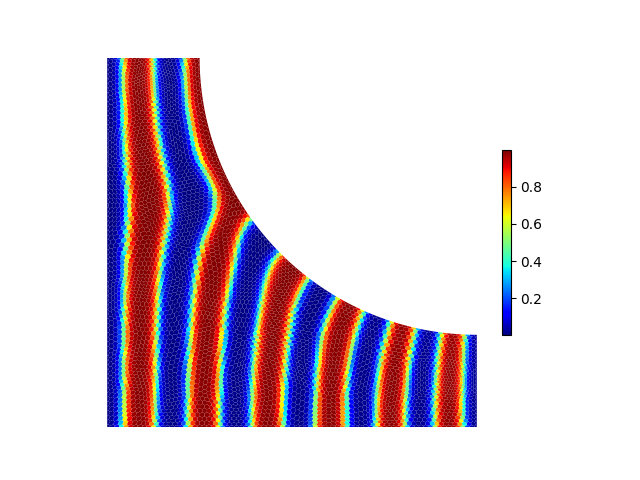
\includegraphics[width=5.2cm]{scftfigure1004.png}
		\caption*{层状相}
	\end{minipage}
\end{figure}
\subsection{不规则区域}   
\begin{table}[H]
	\centering
	\begin{tabular}{cccc}
		\toprule
		区域$D/cm^2$ &	迭代步数 & Q &  H \\
		\midrule
		30*22.5(六状)&340& 3.215353270178076e+02 & -2.093863264593966e+00\\
		30*22.5(层状)&730 &1.461127582677257e+01 & -1.649744476246860e+00\\
		\bottomrule
	\end{tabular}
\end{table}

\begin{figure}[H]
	% 调整字体和图片间距;
	\setlength{\abovecaptionskip}{0.cm}
	\setlength{\belowcaptionskip}{-0.cm}
	% 插入子图;
	\begin{minipage}[!htbp]{0.3\linewidth}
		
\includegraphics[width=5.2cm]{Figure_buming.png}
		\caption*{网格结构}
	\end{minipage}
	\hspace{0.23in}
	\begin{minipage}[!htbp]{0.3\linewidth}
		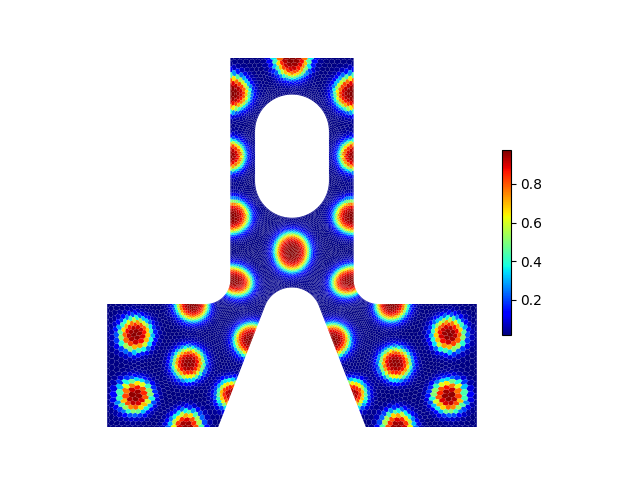
\includegraphics[width=5.2cm]{scftfigure340.png}
		\caption*{六状相}
	\end{minipage}
	\hspace{0.23in}
	\begin{minipage}[!htbp]{0.3\linewidth}
		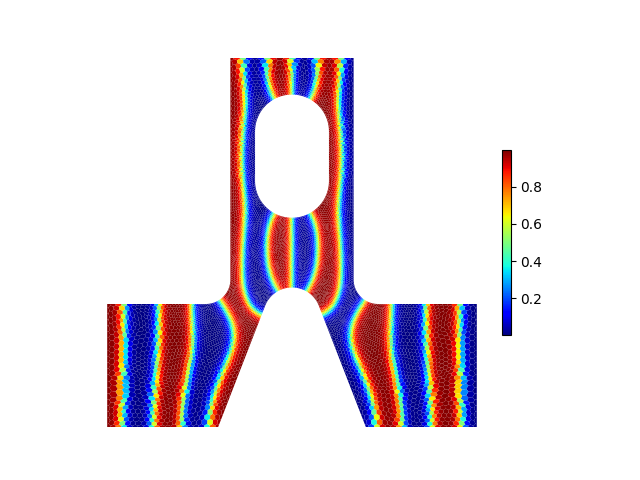
\includegraphics[width=5.2cm]{scftfigure730.png}
		\caption*{层状相}
	\end{minipage}
\end{figure}
\subsection{凹型区域}   
\begin{table}[H]
	\centering
	\begin{tabular}{cccc}
		\toprule
		区域$D/cm^2$ &	迭代步数 & Q &  H \\
		\midrule
		40*24(六状)&770& 2.937431431771336e+02 & -2.371863745147272e+00\\
		40*24(层状)&1163& 2.743809265296202e+00& -1.688270323744312e+00\\
		\bottomrule
	\end{tabular}
\end{table}

\begin{figure}[H]
	% 调整字体和图片间距;
	\setlength{\abovecaptionskip}{0.cm}
	\setlength{\belowcaptionskip}{-0.cm}
	% 插入子图;
	\begin{minipage}[!htbp]{0.3\linewidth}
		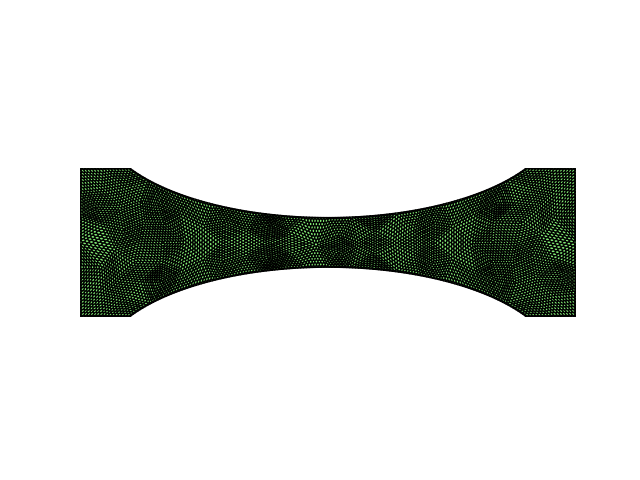
\includegraphics[width=5.2cm]{Figure_ao.png}
		\caption*{网格结构}
	\end{minipage}
	\hspace{0.23in}
	\begin{minipage}[!htbp]{0.3\linewidth}
		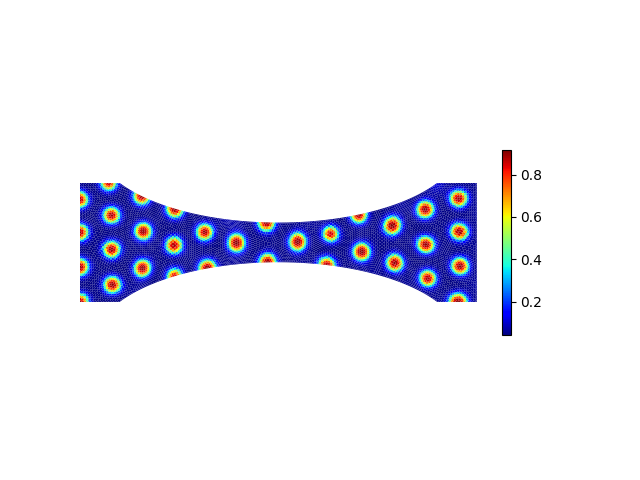
\includegraphics[width=5.2cm]{scftfigure770.png}
		\caption*{六状相}
	\end{minipage}
	\hspace{0.23in}
	\begin{minipage}[!htbp]{0.3\linewidth}
		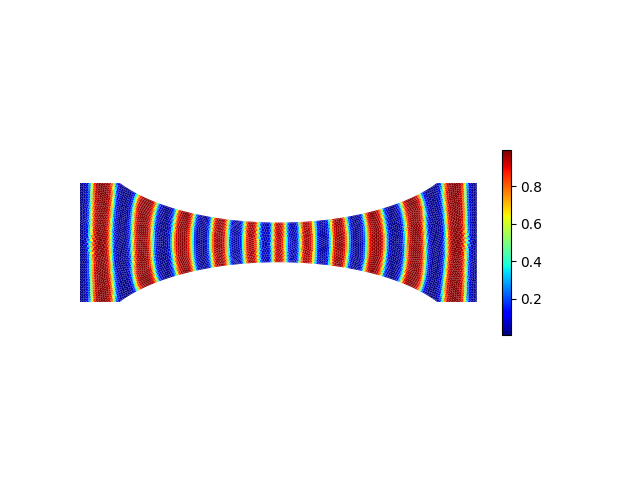
\includegraphics[width=5.2cm]{scftfigure1162.png}
		\caption*{层状相}
	\end{minipage}
\end{figure} 
\subsection{机翼型区域}   
\begin{table}[H]
	\centering
	\begin{tabular}{cccc}
		\toprule
		区域$D/cm^2$ &	迭代步数 & Q &  H \\
		\midrule
		70*7(六状)&484 &2.948668823497224e+02 & -2.362323363741924e+00\\
		70*7(层状)&1502& 2.403979241983159e-05 & -1.734805119606069e+00\\
		\bottomrule
	\end{tabular}
\end{table}

\begin{figure}[H]
	% 调整字体和图片间距;
	\setlength{\abovecaptionskip}{0.cm}
	\setlength{\belowcaptionskip}{-0.cm}
	% 插入子图;
	\begin{minipage}[!htbp]{0.3\linewidth}
		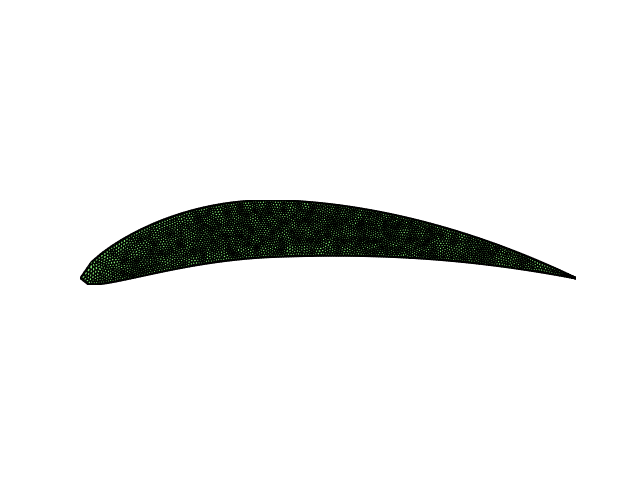
\includegraphics[width=5.2cm]{Figure_air.png}
		\caption*{网格结构}
	\end{minipage}
	\hspace{0.23in}
	\begin{minipage}[!htbp]{0.3\linewidth}
		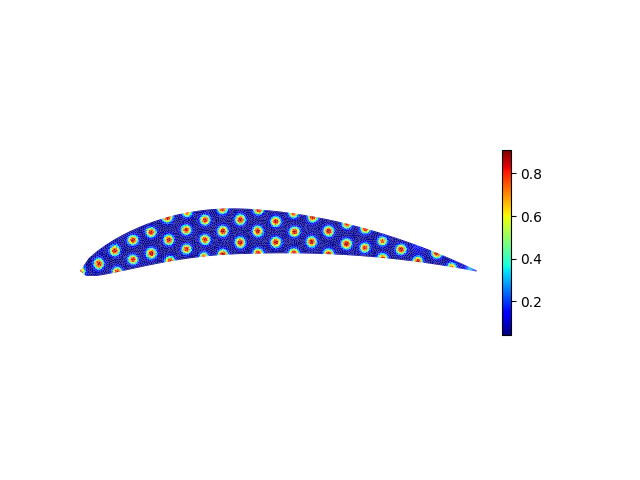
\includegraphics[width=5.2cm]{scftfigure484.png}
		\caption*{六状相}
	\end{minipage}
	\hspace{0.23in}
	\begin{minipage}[!htbp]{0.3\linewidth}
		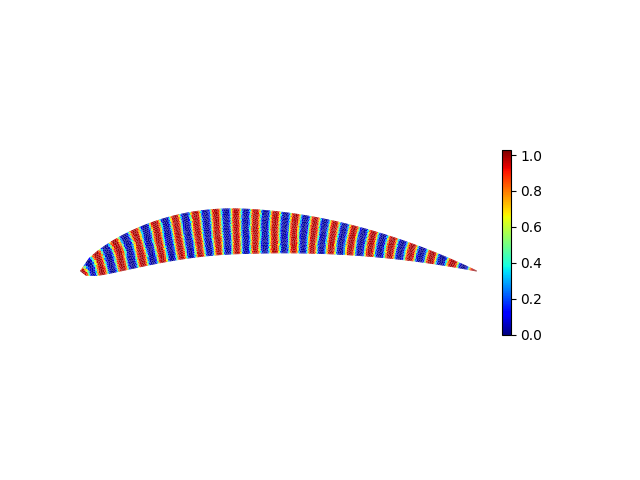
\includegraphics[width=5.2cm]{scftfigure1502.png}
		\caption*{层状相}
	\end{minipage}
\end{figure}    
    
\end{CJK}
\end{document}
